\documentclass{beamer}

% Style
\usepackage{xcolor}

\usetheme{Madrid}
\usepackage{dirtree}
% Color
\definecolor{flatblue}{RGB}{106, 137, 204}
\usecolortheme[named=flatblue]{structure}
% Font
\usepackage{emoji}
\usepackage{fontspec}
\usepackage{csquotes}
\setsansfont{Garamond Libre}
% Code
\usepackage{listings}
\usepackage{graphicx}
\usepackage{hyperref}
\hypersetup{
    colorlinks=true,
    linkcolor=flatblue,
    filecolor=flatblue,
    urlcolor=flatblue,
    citecolor=flatblue
}
\definecolor{flatgreen}{RGB}{0, 98, 102}
\definecolor{flatgreyish}{RGB}{209, 216, 224}
\lstset{
    basicstyle=\ttfamily\scriptsize,
    backgroundcolor=\color{flatgreyish},
    keywordstyle=\color{flatgreen},        % Keywords font ('*' = uppercase)
    commentstyle=\color{flatblue},         % Step between two line-numbers
    columns=fullflexible,
    breaklines=true
}

% Highlight
\usepackage[most]{tcolorbox}
\usepackage{cleveref}
\crefformat{footnote}{#2\footnotemark[#1]#3}
\usepackage{amsmath}
\usepackage{wasysym}
\definecolor{flatorange}{RGB}{255, 165, 2}
\definecolor{flatred}{RGB}{255, 71, 87}
\tcbset{textmarker/.style={%
skin=enhancedmiddle jigsaw,breakable,parbox=false,
boxrule=0mm,leftrule=2mm,rightrule=0mm,boxsep=0mm,arc=0mm,outer arc=0mm,
left=1mm,right=1mm,top=1mm,bottom=1mm,toptitle=1mm,bottomtitle=1mm}}
\newtcolorbox{dangercolorbox}{textmarker,colback=flatorange,colframe=flatred}

% Title
\title{M.E.P. et déploiement - MS2D / ERIS}
\author{Christophe Brun}
\institute{Campus Saint-Michel IT}
\date{17 avril 2024}
\beamertemplatenavigationsymbolsempty

% Graphix with arrows in between
\newcommand*{\vcenterimage}[1]{\vcenter{\hbox{\includegraphics[width=5cm]{#1}}}}
\newcommand*{\vcenterarrow}{\vcenter{\hbox{$\Longrightarrow$}}}

\titlegraphic{
    \bigbreak
    
\includegraphics[width=2cm]{image/logo-papit}
    
\includegraphics[width=2cm]{image/logo-campus-saint-michel-it}
}
\begin{document}

    \begin{frame}
        \transdissolve
        \titlepage
    \end{frame}


    \section{Table des matières}\label{sec:toc}

    \begin{frame}{Table des matières}
        \tableofcontents
    \end{frame}


    \section{Programme du module}\label{sec:programme-du-module}

    \begin{frame}
        \frametitle{Mise en production et déploiement}
        \framesubtitle{Compétence acquise aucours des 5 jours du module}
        \transdissolve
        Compétences~:
        \begin{itemize}
            \item \textquote{Préparer l’environnement et déployer le progiciel ou la solution.}
        \end{itemize}
        \bigbreak
        \centering
        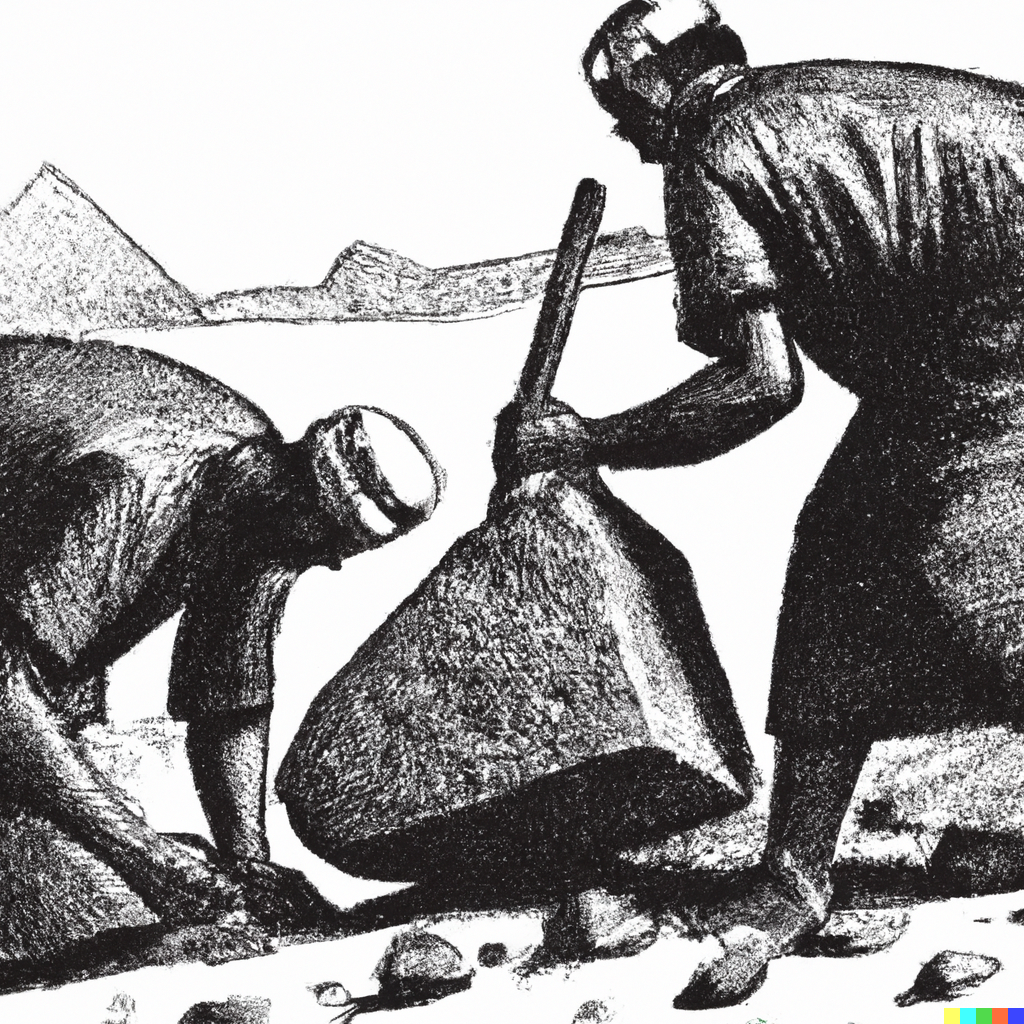
\includegraphics[width=5cm]{image/engraving-of-egyptian-workers-pulling-stones}
    \end{frame}

    \begin{frame}
        \frametitle{Mise en Production et déploiement}
        \framesubtitle{Le programme officiel des 5 jours du module}
        \transdissolve
        \begin{enumerate}
            \item Mise en exploitation des ressources matérielles et logicielles
            \begin{itemize}
                \fontsize{8pt}{8pt}\selectfont
                \item Vérification des configurations
                \item Déploiement des applications
                \item Automatisation des procédures de déploiement
                \item Élaborer les bilans de l’exploitation
                \item Prévoir les évolutions de l’infrastructure
            \end{itemize}
            \item Indicateurs et mesure de performance – Systèmes / Réseau et web
            \begin{itemize}
                \fontsize{8pt}{8pt}\selectfont
                \item Centralisation des journaux et exploitation des logs avec syslogd
                \item Analyse du trafic réseau avec MRTG
                \item Analyse des journaux de type d'Apache Web Server avec Analog
                \item Consolidation d'indicateur de qualité avec rrdtool
                \item Création de page HTML de type tableau de bord avec rrdtool – Tableau de bord
                \item Gestion d’incidents et actions correctives
            \end{itemize}
        \end{enumerate}
    \end{frame}


    \section{Introduction}\label{sec:introduction}

    \begin{frame}
        \transdissolve
        \frametitle{Evaluation}
        \begin{itemize}
            \item Bons et mauvais points tout au long du module.
            \item 80 \% x évaluation continue avec les résultats des exercices.
            \item 20 \% sur une évaluation écrite finale
        \end{itemize}
    \end{frame}

    \begin{frame}
        \transdissolve
        \frametitle{Intervenant sur le module Architecture d'Aplication}
        \framesubtitle{Christophe Brun, conseil en développement informatique}

        \begin{columns}
            \column{0.7\textwidth}
            \begin{itemize}
                \item 1\textsuperscript{ere} année d'intervenant à Saint-Michel \emoji{star-struck}.

                \item 7 ans de conseil en développement au sein d'SSII~.

                \item 7 ans de conseil en développement à mon compte \href{https://papit.fr}{PapIT}.

                \item Passionné~!
                \bigbreak
                \begin{columns}
                    \column{0.5\textwidth}
                    \centering
                    
\includegraphics[width=3cm]{image/logo-uppa}
                    \column{0.5\textwidth}
                    \centering
                    
\includegraphics[width=3cm]{image/logo-universite-bordeaux}
                \end{columns}
            \end{itemize}
            \column{0.3\textwidth}
            \centering
            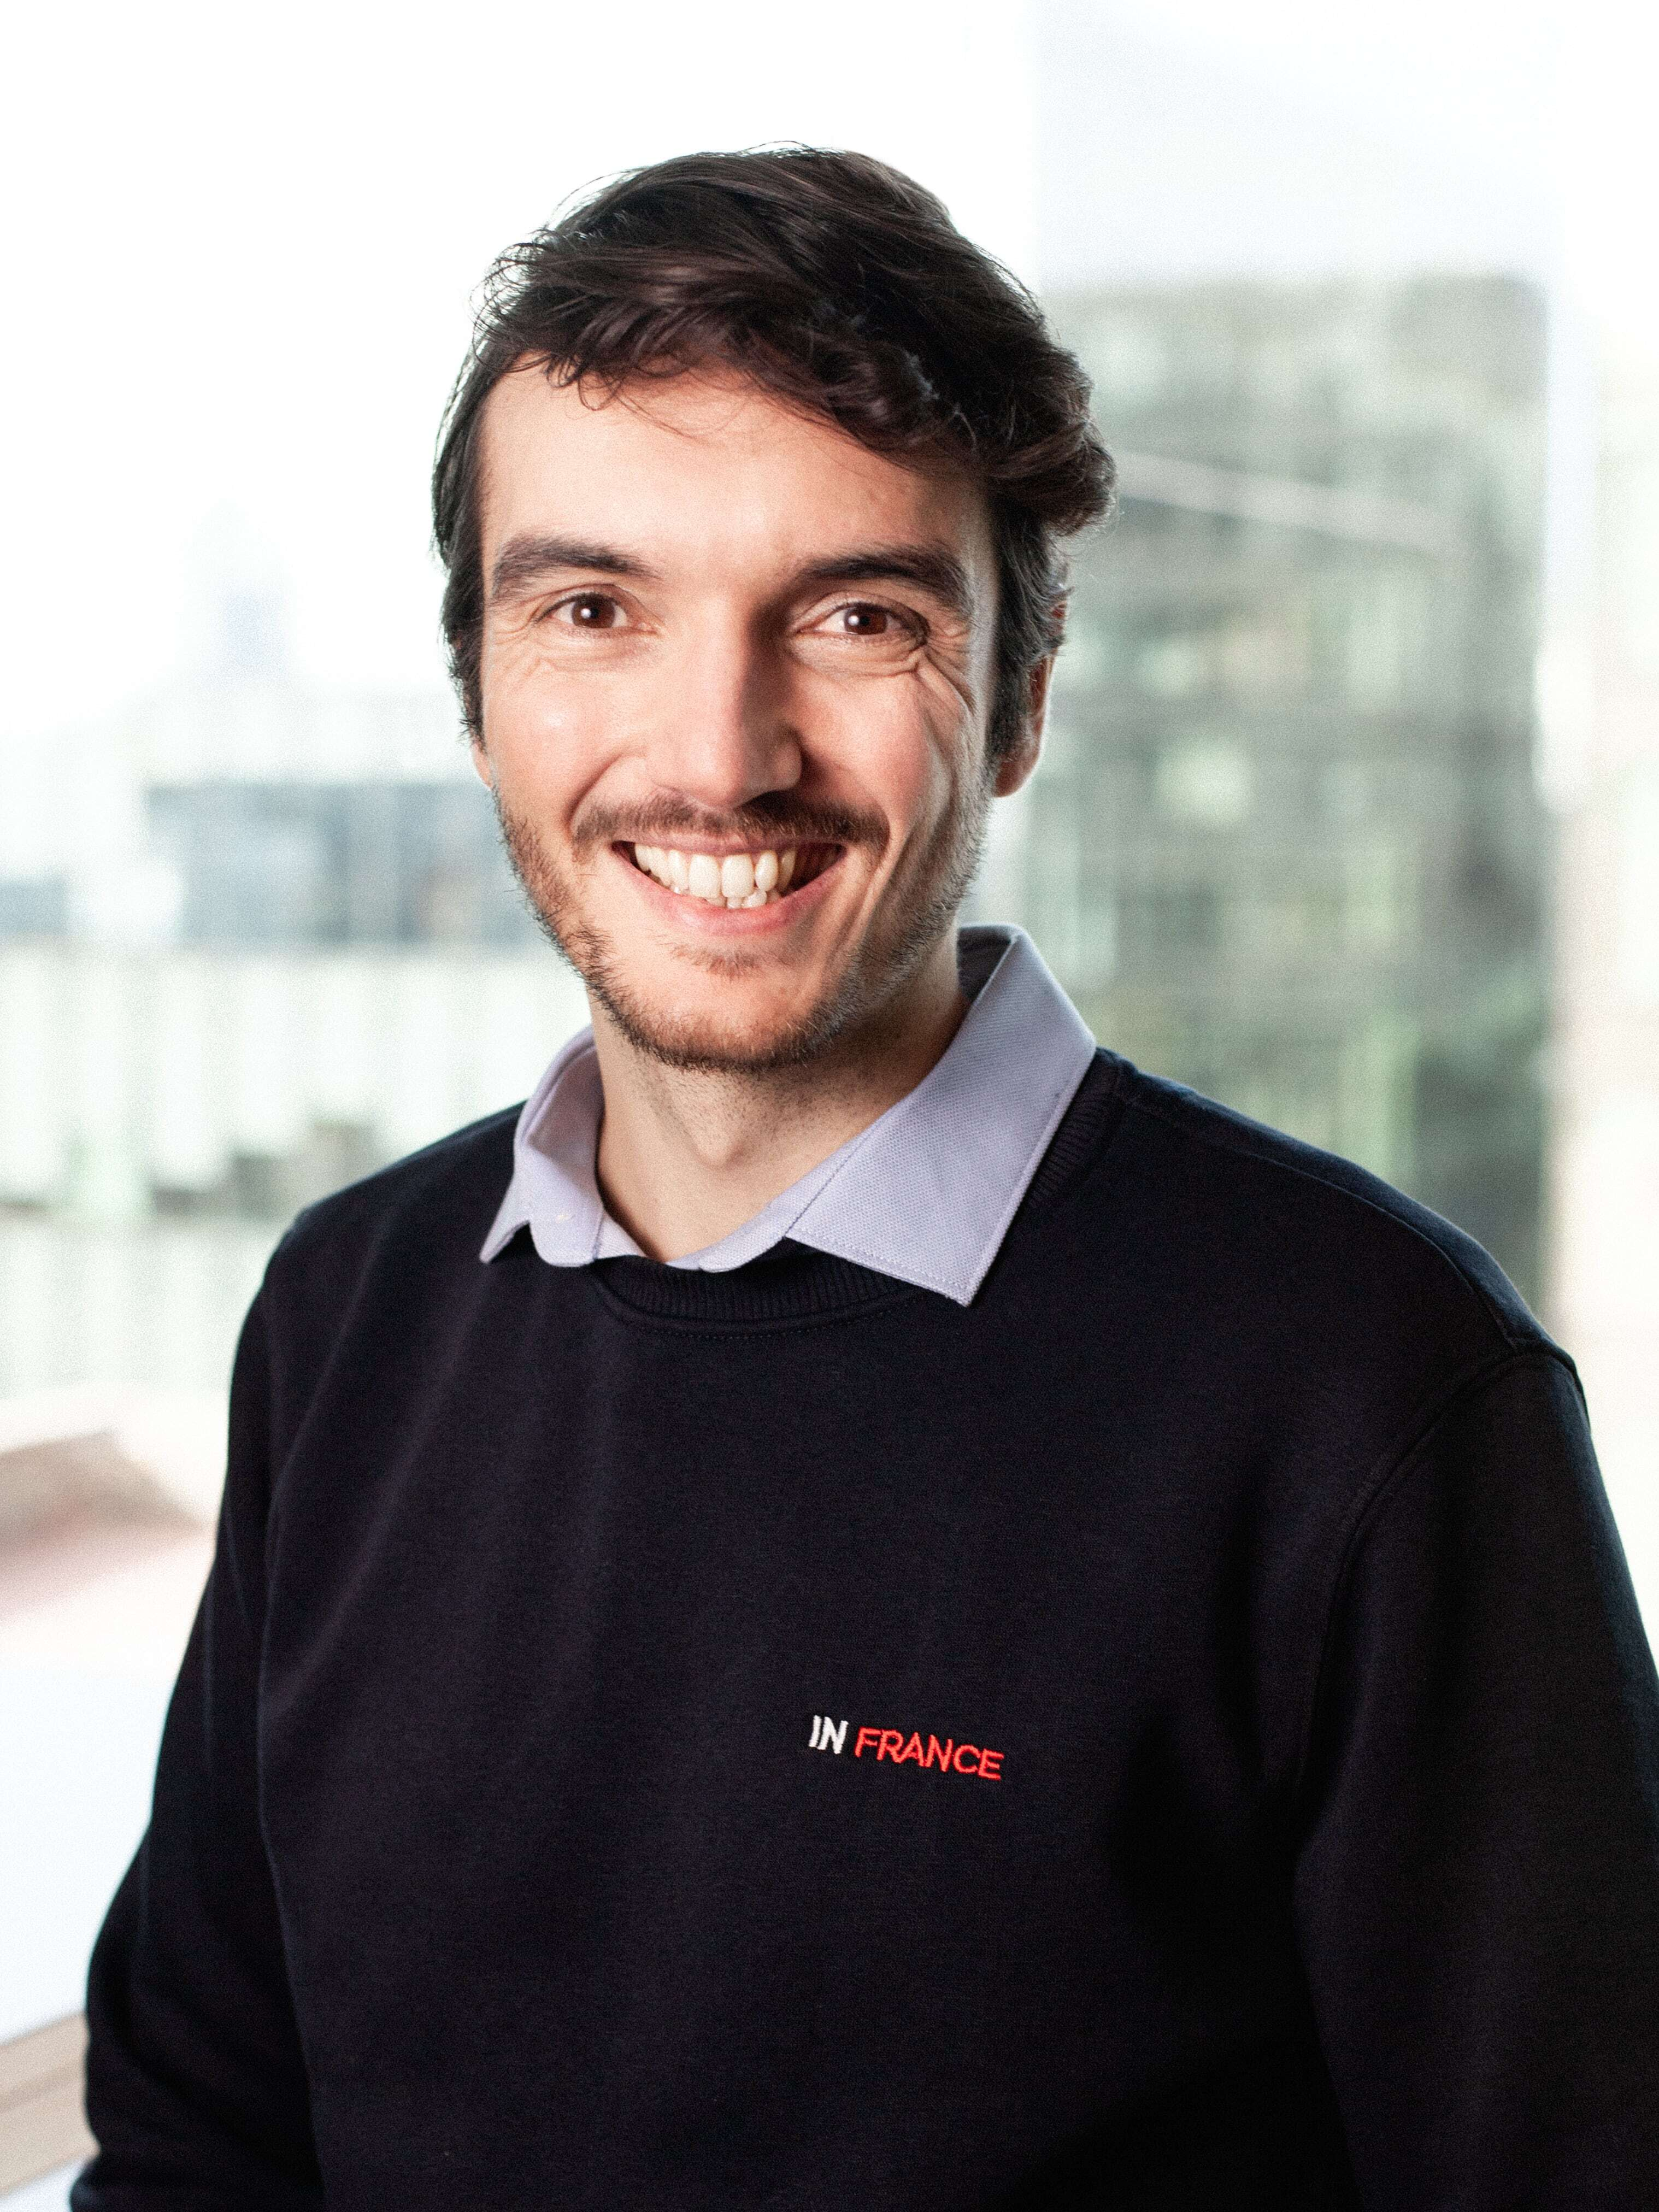
\includegraphics[width=5cm]{image/trombine-christophe}
        \end{columns}
    \end{frame}


    \section{Le matériel}\label{sec:le-materielle}

    \begin{frame}
        \transdissolve
        \frametitle{Les ressources matérielles}
        \framesubtitle{Les machines du web}
        On peut résumer un serveur web à~:
        \begin{itemize}
            \item Un CPU (Architectures x86, ARM, RISC-V, etc.)
            \item De la mémoire RAM
            \item De l'IO
            \begin{itemize}
                \item Disque dur (NVMe)
                \item Réseau (Ethernet, optique)
                \item Disque DVD
            \end{itemize}
        \end{itemize}
        A l'imagine de n'importe quel ordinateur, mais souvent avec plus de capacités et de redondances.
    \end{frame}


    \section{Le logiciel}\label{sec:le-logiciel}

    \begin{frame}
        \transdissolve
        \frametitle{Les ressources logicieles}
        \framesubtitle{Les stacks du web}
        Une stack web est faite en général de~:
        \begin{itemize}
            \item Un OS, qui est une couche d'abstraction du hardware présenté précédemment (Ubuntu, Red Hat, Windows, BSD).
            \item Un reverse Proxy (Apache, Nginx, etc.)
            \item Un serveur web (Apache, Nginx, Gunicorn, NextJS, etc.)
            \item L'application web un ensemble de \textquote{Business rules} implémentées grâce à des bases de données, des IHM, des connections aux API (en PHP, Python, NodeJS, etc.)
            \item Une base de données (MySQL, PostgreSQL, MongoDB, etc.)
        \end{itemize}
    \end{frame}


    \section{Le ressources partagées}\label{sec:le-ressources-partagees}

    \begin{frame}
        \transdissolve
        \frametitle{Les ressources partagées}
        \framesubtitle{Les machines du web}
        Dans un environnement de production, on retrouve une forte variabilité des ressources CPU mais surtout des ressources logicielles.
        \bigbreak
        A cette variabilité des environments de production, il faut ajouter la variabilité des environnements de développement.

        Beaucoup de développeurs travaillent sous Windows ou Mac OS qui sont rarement des environnements de production.
        Les capacités hardware sont souvent très différentes, la production a plus de capacité que le développement en général.
        \bigbreak
        C'est cette variabilité des environnements qui est la difficulté majeur du déploiement et de la mise en production.
    \end{frame}

    \begin{frame}
        \transdissolve
        \frametitle{Les ressources partagées}
        \framesubtitle{Les environnements cloud}
        Pour palier à cette variabilité, diverses architectures en nuage ont vu le jour.

        Certaines ont abstraient le hardware voir même une partie du software pour ne laisser que l'application.
        \bigbreak
        \centering
        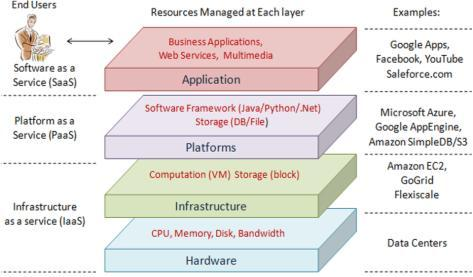
\includegraphics[width=6cm]{image/cloud-stacks} \\ IAAS, PAAS et SAAS\\
        \flushleft
        On voit que SAAS et Paas ont fait abstraction du hardware\footnote{\label{arcuscloud}Patel et al., \url{https://www.researchgate.net/publication/324692035_Arcus_Cloud_A_Private_Cloud_Establishment}}.
    \end{frame}

    \begin{frame}
        \transdissolve
        \frametitle{Les ressources partagées}
        \framesubtitle{Les environnements cloud}
        \begin{dangercolorbox}
            Abstraction du hardware ne veut plus dire qu'on a plus du tout besoin de s'en soucier.
            Même dans le cloud public il faut adapter les capacités des ressources aux besoins et aux coûts.
        \end{dangercolorbox}
        \begin{columns}
            \column{0.5\textwidth}
            \centering
            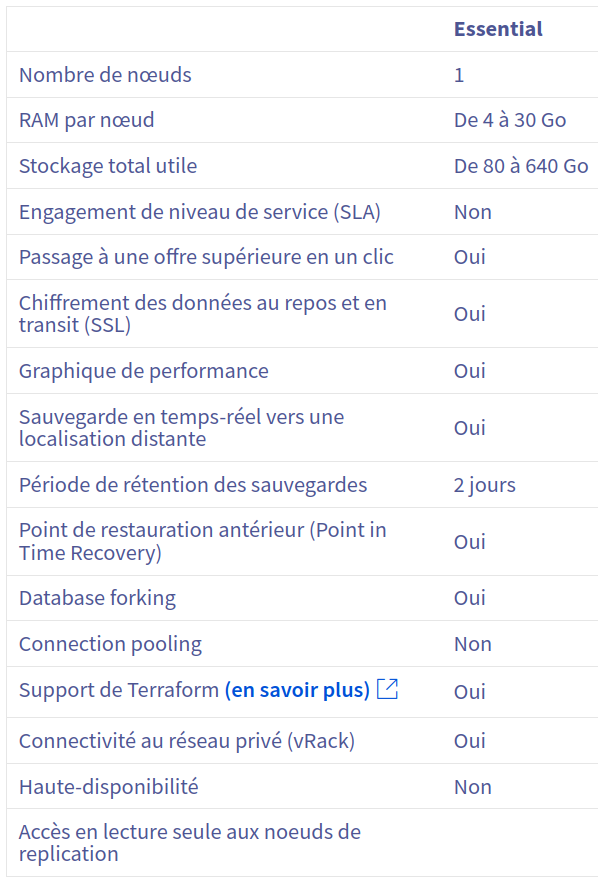
\includegraphics[width=3cm]{image/ovh-public-mysql} \\ MySQL sur le cloud public OVH \\
            \column{0.5\textwidth}
            \centering
            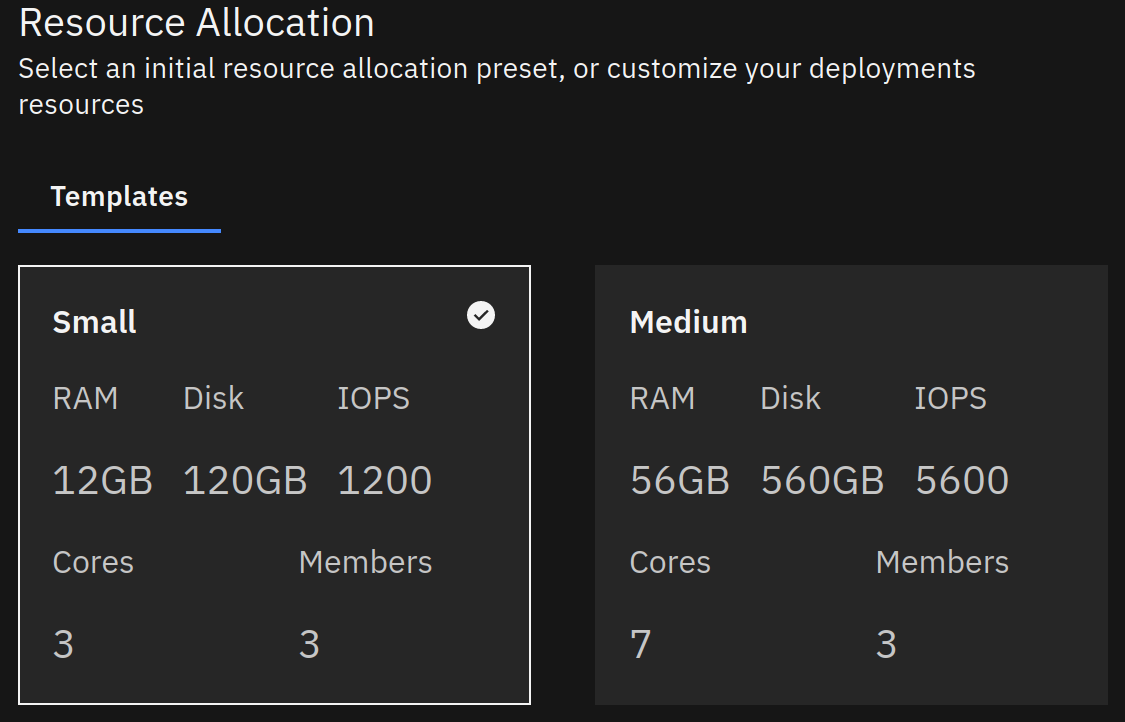
\includegraphics[width=5cm]{image/ibm-public-mysql} \\ MySQL sur le cloud public IBM \\
        \end{columns}
        \flushleft
        \bigbreak
        Qu'est-ce qui vous étonne dans ces deux captures d'écran ?
    \end{frame}

    \begin{frame}
        \transdissolve
        \frametitle{Les ressources partagées}
        \framesubtitle{Les environnements cloud}

        Le cloud public donne souvent l'impression que les ressources sont infinies, mais c'est faux.

        Ils ne communiquent même pas les métriques requises pour comprendre les capacités de leur cloud.

        \bigbreak
        Le cloud privé à l'avantage de présenter de manière plus claire les ressources hardware.
    \end{frame}

    \begin{frame}
        \transdissolve
        \frametitle{Les ressources partagées}
        \framesubtitle{Les environnements cloud}
        Même dans le cloud privé, les vCPU ne sont pas des CPU physiques, mais des CPU partagés.

        Ce n'est indiqué nul part, mais c'est probablement le cas chez OVH~.
        Cela implique que OS qui héberge l'hyperviseur équilibre en permanence les ressources CPU entre les VM~.
        Cela a un coût en performance qui est inconnu.
        \bigbreak
        Techniquement ce n'est pas obligatoire de partager les CPU, mais c'est souvent le cas pour des raisons de scalabilité.
        Au besoin un coeur physique peut être dédié à une seule VM~.
        \bigbreak
        Linode, un cloud provider, apporte des informations claires sur ce sujet \url{https://www.linode.com/docs/products/compute/compute-instances/plans/comparing-shared-and-dedicated-cpus/}.

    \end{frame}

    \begin{frame}
        \transdissolve
        \frametitle{Les ressources partagées}
        \framesubtitle{La virtualisation}
        Développée par IBM dès les années 60, la virtualisation permet de créer plusieurs machines virtuelles sur un seul hardware.
        Elle fut d'abord commercialement disponible sur les mainframes avant les plus petites plateformes AS400, iSeries et Power.
        Le technologie TIMI d'IBM permet depuis les années 80 de faire tourner des programmes qui restent compatibles avec des hardwares de plus en plus puissants (changement d'ISA, d'\textit{endianness} A.K.A boutisme en français).
        \bigbreak
        Cela permet de mutualiser les ressources hardware, de les partager en fonction des besoins et même de changer de hardware.
        \bigbreak
        Elle apporte un gain de sécurité en isolant les VM les unes des autres.
        \begin{dangercolorbox}
            Quid des gros bugs /failles de sécurité comme Meltdown et Spectre ?
        \end{dangercolorbox}
    \end{frame}

    \begin{frame}
        \transdissolve
        \frametitle{Les ressources partagées}
        \framesubtitle{La virtualisation\cref{arcuscloud}}
        Aujourd'hui la virtualisation est principalement utilisée pour le partage des ressources et isoler les applications dans une VM pour raison de sécurité.
        Un OS hôte fait tourner un hyperviseur qui lui fait tourner des VM et plus juste un soft compilé.
        \bigbreak
        \centering
        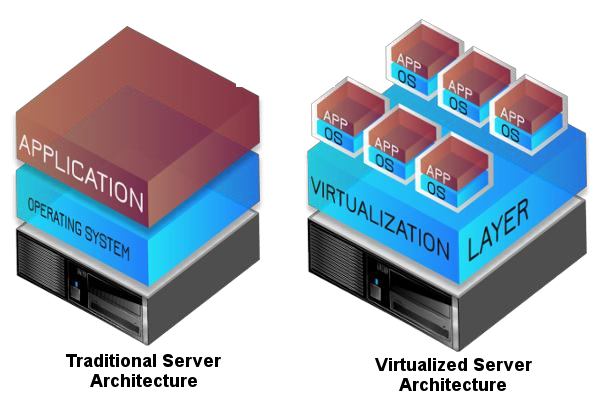
\includegraphics[width=6cm]{image/virtualisation}
    \end{frame}

    \begin{frame}
        \transdissolve
        \frametitle{Les ressources partagées}
        \framesubtitle{La virtualisation avec KVM et Qemu\footnote{\label{ubuntukvm}KVM hypervisor: a beginners’ guide, \url{https://ubuntu.com/blog/kvm-hyphervisor}]}}
        \begin{columns}
            \column{0.5\textwidth}
            KVM (Kernel-based Virtual Machine) est une technologie de virtualisation ouverte intégrée à Linux.

            C'est un hyperviseur de type 1, qui négocie directement avec le hardware et offre des performances proches de la machine hôte.
            Contrairement à un hyperviseur de type 2, qui doit passer par l'OS hôte pour accéder au hardware mais ces derniers ont donc une meilleurs portabilité et compatibilité.
            \column{0.5\textwidth}
            \centering
            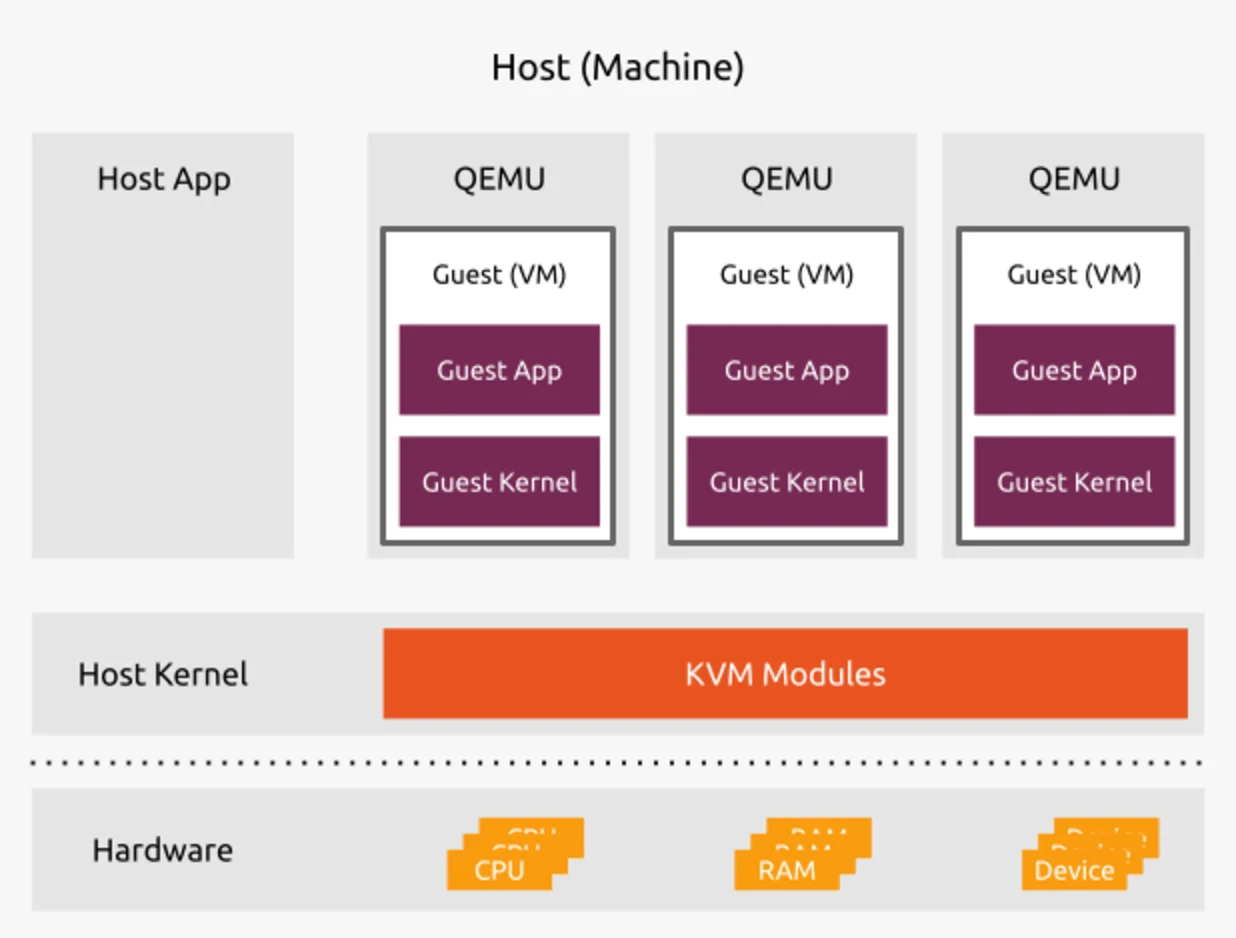
\includegraphics[width=6cm]{image/kvm-qemu}
        \end{columns}
        \bigbreak
        Qemu lui peut faire tourner des VM avec ou sans KVM en fonction des besoins.
    \end{frame}

    \begin{frame}
        \transdissolve
        \frametitle{Les ressources partagées}
        \framesubtitle{Exercice, avec ou sans KVM~?}
        \begin{columns}
            \column{0.5\textwidth}
            \begin{itemize}
                \item Un Windows guest sur un Mac OS hôte?
                \item Un Alpine Linux sur un Raspberry\footnotemark~?
                \item VM Ubuntu sur un Ubuntu hôte?
                \item VM Ubuntu sur un Windows hôte?
            \end{itemize}
            \column{0.5\textwidth}
            \centering
            
\includegraphics[width=6cm]{image/question-mark-on-a-blank-background}
        \end{columns}
        \footnotetext{\url{https://unix.stackexchange.com/questions/340912/qemu-with-kvm-with-differaing-host-guest-architectures}}
    \end{frame}


    \section{Les services}\label{sec:les-services}

    \begin{frame}
        \transdissolve
        \frametitle{Les services}
        \framesubtitle{Définition}
        Dans les systèmes Windows et Linux, le terme service désigne un programme qui s'exécute en arrière-plan, sans intervention de l'utilisateur.

        Il faut le configurer pour qu'il démarre automatiquement, dans un certain ordre et avec les bonnes permissions.
        \bigbreak
        La configuration principale consiste à définit une ligne de commande qui sera exécutée au démarrage du service.
        \bigbreak
        Avec \lstinline{systemd}\footnote{System and Service Manager, \url{https://systemd.io/}} sous Linux, on peut définir des dépendances entre les services.
        Limiter les ressources CPU, mémoire, IO, etc.
        Définir ce qu'il faut faire en cas de crash.
        Exécuter des scripts avant et après le démarrage du service.
        \bigbreak
        Leur chemin par défaut est \lstinline{/etc/systemd/system/}.
        \begin{dangercolorbox}
            Ne pas confondre \lstinline{systemd} qui exécute des tâches en arrière plan et l'ordonnanceur \lstinline{cron}.
        \end{dangercolorbox}
    \end{frame}

    \begin{frame}[fragile]
        \transdissolve
        \frametitle{Les services}
        \framesubtitle{Examples}
        \lstinline{systemd} est donc l'outil de choix pour lancer en production des applications, des progiciels, etc.

        Encore mieux, on peut configurer des services pour qu'ils lancent des VM avec Qemu et les applications tourneraient dans les VM~.
        On profites des avantages de la virtualisation pour isoler les applications et les sécuriser.
        \bigbreak
        Que fait cette configuration~?
        \begin{lstlisting}
[Unit]
Description=IN DATA development application
[Service]
RuntimeMaxSec=3600s
Restart=always
WorkingDirectory=/home/debian/dev/IN FRANCE
ExecStart="/home/debian/dev/IN FRANCE/python3-dev/bin/python3" -m gunicorn -w 1 -b unix:/tmp/in-france-dev-indata-gunicorn.sock application_indata
[Install]
WantedBy=multi-user.target
        \end{lstlisting}
        \begin{dangercolorbox}
            Le chemin de l'exécutable dans \lstinline{ExecStart} doit être absolu!
        \end{dangercolorbox}
    \end{frame}

    \begin{frame}
        \transdissolve
        \frametitle{Les services}
        \framesubtitle{Les commandes de base}
        \begin{itemize}
            \item \lstinline{systemctl start <service>} pour démarrer un service.
            \item \lstinline{systemctl stop <service>} pour arrêter un service.
            \item \lstinline{systemctl restart <service>} pour redémarrer un service.
            \item \lstinline{systemctl status <service>} pour afficher le statut d'un service.
            \item \lstinline{systemctl enable <service>} pour activer un service au démarrage.
            \item \lstinline{systemctl disable <service>} pour désactiver un service au démarrage.
            \item \lstinline{systemctl list-units --type=service} pour lister les services.
            \item \lstinline{systemctl daemon-reload} pour recharger la configuration de tous les services.
            \item \lstinline{systemctl reload <service>} pour recharger la configuration d'un service.
        \end{itemize}
    \end{frame}
    \begin{frame}
        \transdissolve
        \frametitle{Les services}
        \framesubtitle{Les commandes pour monitorer l'exécution}
        Pour monitor les logs d'un service, la commande \lstinline{journalctl} est très utile.
        \bigbreak
        Quelques exemples de commandes utiles~:
        \begin{itemize}
            \item \lstinline{journalctl --unit<service>} pour afficher les logs d'un service.
            \item \lstinline{journalctl --unit<service> -f} pour afficher les logs en temps réel.
            \item \lstinline{journalctl --unit<service> --since "2024-04-17 00:00:00"} pour afficher les logs depuis une date.
            \item \lstinline{journalctl --unit<service> --since "2024-04-17 00:00:00" --until "2024-04-17 23:59:59"} pour afficher les logs entre deux dates.
            \item \lstinline{journalctl --unit=<service> -n 100 --no-pager} pour afficher les 100 dernière lignes.
        \end{itemize}
    \end{frame}

    \begin{frame}
        \transdissolve
        \frametitle{Exercice pratique}
        \framesubtitle{Créer une VM avec Qemu et lancer une application avec systemd}
        Les exigences~:
        \begin{itemize}
            \item Créer une VM Linux avec Qemu à l'image d'un VPS OH d'entrée de gamme (1~vCPU, 2~Go de RAM et 10~Go de disque).
            \item Configurer la machine hôte pour démarrer la VM automatiquement.
            \item Configurer la VM et Qemu avec une sécurité en accord les bonnes pratiques de sécurité (Clé SSH uniquement, pas de connexion SSH avec le user root, gestion des ports forwardés).
            \item Démarrer l'application Gunicorn \textquote{Hello World} \url{https://gunicorn.org/\#quickstart} avec \lstinline{systemd}.
            \item Accès à la VM et à l'application depuis la machine hôte.
        \end{itemize}
    \end{frame}

    \begin{frame}[fragile]
        \transdissolve
        \frametitle{Exercice pratique}
        \framesubtitle{Une des solutions (commandes à exécuter sur la machine hôte)}
        \begin{lstlisting}[language=bash]
qemu-img create -f qcow2 linux.qcow2 10G # Create a disk image
# Download a minial Ubuntu ISO
wget http://archive.ubuntu.com/ubuntu/dists/bionic/main/installer-amd64/current/images/netboot/mini.iso
# Install the OS using a virtual CDROM
qemu-system-x86_64 -m 2G -smp 1 -nic user -boot d -cdrom mini.iso -hda linux.qcow2 -k fr -enable-kvm
# Run the VM to configure and test SSH
qemu-system-x86_64 -m 2G -smp 1 -nic user,hostfwd=tcp::5022-:22,hostfwd=tcp::5080-:80 -display none -hda linux.qcow2 -k fr -enable-kvm
        \end{lstlisting}
        Expliquez chacune des lignes de commande ci-dessus.
        \bigbreak
        Ressources utiles~:
        \begin{itemize}
            \item \href{https://wiki.alpinelinux.org/wiki/Install_Alpine_in_QEMU}{Similaire mais avec Alpine Linux}
            \item \href{https://help.ubuntu.com/community/Installation/MinimalCD\#A64-bit_PC_.28amd64.2C_x86_64.29_.28Recommended.29}{Page d'installation Ubuntu du \textquote{MinimalCD} }
            \item \href{https://phoenixnap.com/kb/generate-setup-ssh-key-ubuntu}{Configuration des login SSH sur Ubuntu}
        \end{itemize}
    \end{frame}

    \begin{frame}[fragile]
        \transdissolve
        \frametitle{Exercice pratique}
        \framesubtitle{Une des solutions}
        Le service de la machine hôte~:
        \begin{lstlisting}[language=bash]
[Unit]
Description=Qemu Ubuntu VM for St-Michel classes
After=network.target
StartLimitIntervalSec=0

[Service]
Restart=always
WorkingDirectory=/home/chrichri/Documents/Campus-St-Michel-IT/production-deployment
ExecStart=/usr/bin/qemu-system-x86_64 -m 2G -smp 1,maxcpus=1 -nic user,hostfwd=tcp::5022-:22,hostfwd=tcp::5080-:8080 -display none -hda linux.qcow2 -k fr -enable-kvm

[Install]
WantedBy=multi-user.target
        \end{lstlisting}
        Expliquez chaque option de la configuration du service.
        \pause
        \begin{dangercolorbox}
            \lstinline{-enable-kvm} si l'hôte est un Linux également.

            \lstinline{-display none} pour ne pas afficher la console graphique.
        \end{dangercolorbox}
    \end{frame}

    \begin{frame}[fragile]
        \transdissolve
        \frametitle{Exercice pratique}
        \framesubtitle{Une des solutions}
        Le service dans la VM~:
        \begin{lstlisting}[language=bash]
[Unit]
Description=St-Michel Hello World
After=network.target
StartLimitIntervalSec=0

[Service]
Restart=always
WorkingDirectory=/home/chrichri
ExecStart=/usr/bin/gunicorn -w 1 hello:app -b 0.0.0.0:8080

[Install]
WantedBy=multi-user.target
        \end{lstlisting}
        Expliquez chaque option de la configuration du service.
    \end{frame}

    \begin{frame}[fragile]
        \transdissolve
        \frametitle{Exercice pratique}
        \framesubtitle{Une des solutions (commande à exécuter sur la VM)}
        Commande pour configurer la VM~:
        \begin{lstlisting}[language=bash]
# Install gunicorn, pip install gunicorn is no longer recommanded
sudo apt-get install python3-gunicorn
# Configure SSH
sudo sed -i 's/PermitRootLogin yes/PermitRootLogin no/' /etc/ssh/sshd_config
sudo sed -i 's/PasswordAuthentication yes/PasswordAuthentication no/' /etc/ssh/sshd_config
# Restart SSH with the new configuration
sudo systemctl restart sshd
# Create the .ssh directory and the authorized_keys file
mkdir -p ~/.ssh
touch ~/.ssh/authorized_keys
# Add the public key to the authorized_keys file
echo "ssh-rsa AAAAB3NzaC1yc2EAAAADAQABAAABgQDQ8z4... chrichri@localhost" >> ~/.ssh/authorized_keys
        \end{lstlisting}
        Expliquez chaque commande.
    \end{frame}


    \section{Ansible}\label{sec:ansible}

    \begin{frame}
        \transdissolve
        \frametitle{Automatisation de la configuration avec Ansible}
        \framesubtitle{Définition\footnote{Ansible Community Documentation, \url{https://docs.ansible.com/ansible/latest/getting_started/index.html}}}
        Ansible est un outil d'automatisation de la configuration des machines physiques ou virtuelles.
        Il permet de définir des \textquote{playbooks} qui décrivent une configuration à appliquer aux machines qui sont dans l'\textquote{inventory} .
        \bigbreak
        \centering
        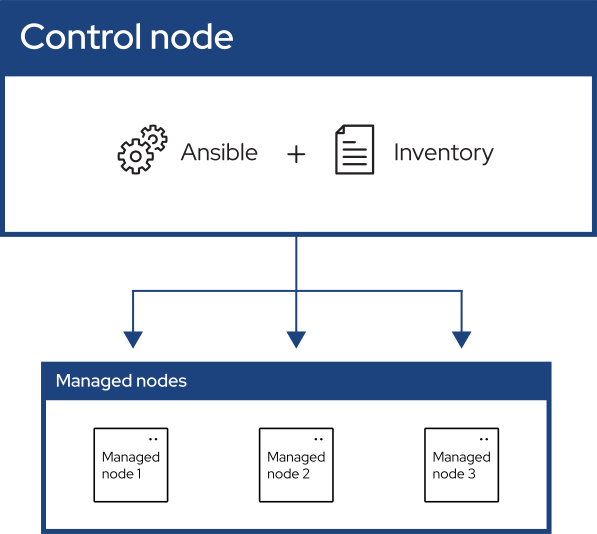
\includegraphics[width=5cm]{image/ansible}
    \end{frame}

    \begin{frame}[fragile]
        \transdissolve
        \frametitle{Automatisation de la configuration avec Ansible}
        \framesubtitle{Example d'inventaire}
        Pour accéder à la VM créée précédemment dans Qemu, il faut définir un inventaire avec les données dont on aurait besoin pour y accéder en SSH~.
        \begin{lstlisting}[language=bash]
$ ssh chrichri@localhost -p 5022 -v -i /home/chrichri/Documents/Campus-St-Michel-IT/production-deployment/virt-ubuntu
        \end{lstlisting}
        La commande ci-dessus, devient dans l'inventaire (on peut créer des variables)~:
        \begin{lstlisting}
[gunicorn]
localhost:5022 ansible_ssh_private_key_file=/home/chrichri/Documents/Campus-St-Michel-IT/production-deployment/virt-ubuntu ansible_ssh_user=chrichri
        \end{lstlisting}
        On utilise le module \lstinline{ping} pour vérifier que l'accès SSH est correctement configuré.
        \begin{lstlisting}[language=bash]
$ ansible gunicorn -m ping -i inventory.ini
localhost | SUCCESS => {
    "ansible_facts": {
        "discovered_interpreter_python": "/usr/bin/python3"
    },
    "changed": false,
    "ping": "pong"
}
        \end{lstlisting}
    \end{frame}

    \begin{frame}
        \transdissolve
        \frametitle{Automatisation de la configuration avec Ansible}
        \framesubtitle{Aucune installation côté client\emoji{heart}}
        Pourquoi Ansible n'a aucun client sur les machines de l'inventaire~?
        \bigbreak
        \centering
        
\includegraphics[width=5cm]{image/question-mark-on-a-blank-background}
        \bigbreak
        \pause
        \flushleft
        Avec le seul accès SSH, il exécute les commandes qu'il faut.
        Il est agnostique à l'OS~!
    \end{frame}

    \begin{frame}[fragile]
        \transdissolve
        \frametitle{Automatisation de la configuration avec Ansible}
        \framesubtitle{Example de \textquote{playbook}}
        Qu'a-t-on installé sur un Ubuntu \textit{base server} comme package(s) pour pouvoir exécuter l'application gunicorn Hello World~?
        \pause
        % With apt, packages python3-gunicorn
        \begin{lstlisting}[language=bash]
sudo apt-get install python3-gunicorn
        \end{lstlisting}
        Commande qui devient dans un playbook Ansible \lstinline{gunicorn.yml}~:
        \begin{lstlisting}
---
- name: gunicorn
  hosts: gunicorn
  become: yes # Run as root
  tasks:
  - name: Install gunicorn
    apt:
      name: gunicorn # Le package à installer
      state: present
        \end{lstlisting}
        À lancer avec la commande~:
        \begin{lstlisting}[language=bash]
$ ansible-playbook -i inventory.ini gunicorn.yml
        \end{lstlisting}
    \end{frame}

    \begin{frame}[fragile]
        \transdissolve
        \frametitle{Automatisation de la configuration avec Ansible}
        \framesubtitle{Example de \textquote{playbook}}
        Le résultat de l'exécution du playbook \lstinline{gunicorn.yml}~:
        \begin{lstlisting}[language=bash]
$ ansible-playbook -i inventory.ini gunicorn.yml
...
localhost                  : ok=2    changed=1    unreachable=0    failed=0    skipped=0    rescued=0    ignored=0

$ ansible-playbook -i inventory.ini gunicorn.yml
...
localhost                  : ok=2    changed=0    unreachable=0    failed=0    skipped=0    rescued=0    ignored=0
        \end{lstlisting}
        A la première exécution, le package est installé, à la seconde il est déjà installé, aucun changement.
    \end{frame}

    \begin{frame}[fragile]
        \transdissolve
        \frametitle{Automatisation de la configuration avec Ansible}
        \framesubtitle{Commande pour exécuter un programme}
        Une fois les dépendances requises installées, on peut exécuter un programme avec le module \lstinline{shell}~.
        \bigbreak
        Si il faut copier un ou plusieurs fichiers, on peut utiliser le module \lstinline{copy}~.
        \bigbreak
        Par exemple~:
        \begin{lstlisting}
---
- hosts: gunicorn # Groupe de host de l'inventory
  vars:
  - EXEC_ABS_PATH: /home/chrichri/helloworld # Utilisé 2 fois donc dans une variable
...
  - name: Copy Application
    copy:
      src: /home/chrichri/Documents/Campus-St-Michel-IT/production-deployment/helloworld/build/helloworld # Le build de ma machine
      dest: "{{ EXEC_ABS_PATH }}"

  - name: Run Application
    shell: nohup {{ EXEC_ABS_PATH }} & # nohup pour exécuter en arrière plan
        \end{lstlisting}
    \end{frame}

    \begin{frame}
        \transdissolve
        \frametitle{Automatisation de la configuration avec Ansible}
        \framesubtitle{La Ansible Galaxy}
        Comme souvent, inutile de tout recoder.
        Ansible est modulaire grâce aux \textquote{roles} et aux \textquote{playbooks} qui sont eux-mêmes des modules\footnote{Roles, \url{https://docs.ansible.com/ansible/latest/playbook_guide/playbooks_reuse_roles.html}}.
        \bigbreak
        La communauté Ansible a packagé des modules et des playbooks pour les tâches les plus courantes\footnote{Ansible Galaxy, \url{https://galaxy.ansible.com/ui/}}.
        Ils sont disponibles sur la \href{https://galaxy.ansible.com/}{Ansible Galaxy}.
        Et peuvent être installés avec la commande \lstinline{ansible-galaxy install <module>}, commande issue du package \lstinline{ansible-core}.
    \end{frame}

    \begin{frame}
        \transdissolve
        \frametitle{Automatisation de la configuration avec Ansible}
        \framesubtitle{Ansible et Windows}
        Sur la machine hôte, on ne peut l'installer que depuis un WSL~.
        \begin{dangercolorbox}
            Si la machine cliente est un Windows, attention au package manager et aux séparateurs de chemin, voir \url{https://docs.ansible.com/ansible/latest/os_guide/windows_usage.html}.
        \end{dangercolorbox}
        \bigbreak
        \centering
        
\includegraphics[width=5cm]{image/broken-windows} \\ L'idéal reste quand même de ne pas utiliser Windows\ldots \\
    \end{frame}

    \begin{frame}
        \transdissolve
        \frametitle{Automatisation de la configuration avec Ansible}
        \framesubtitle{Excercice}
        En utilisant la VM crée à l'exercice précédent, configurer un inventaire et un playbook pour installer l'application Spring Boot.
        \bigbreak
        Vous pouvez vous aider du \href{https://spring.io/guides/gs/spring-boot}{tutoriel officiel}.
        \bigbreak
        \centering
        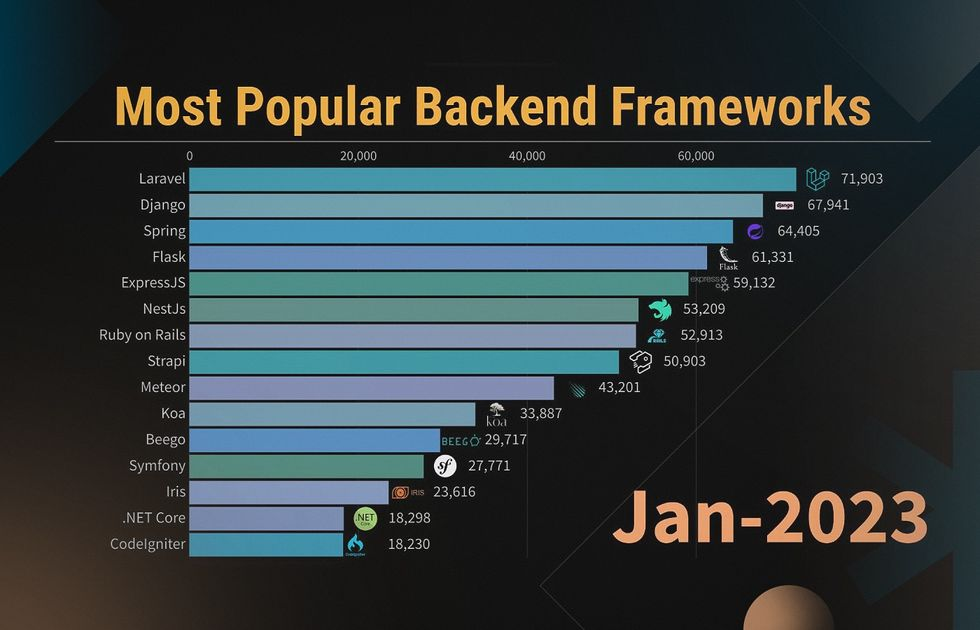
\includegraphics[width=8cm]{image/most-popular-backend}
    \end{frame}

    \begin{frame}
        \transdissolve
        \frametitle{Automatisation de la configuration avec Ansible}
        \framesubtitle{Solution à l'exercice}
        De nombreuses solutions sont valides.
        Mais avec Java il est plus simple de profiter du \textquote{Write once, run anywhere}.
        \bigbreak
        Ce n'est donc pas obliger d'utiliser un système de build comme Maven ou Gradle sur la VM, Java suffit pour exécuter une JAR~.
        \bigbreak
        Une JAR (Java ARchive) est un exécutable qui contient toutes les classes zippées et qui se lance avec \lstinline{java -jar <JAR file>}.
        Il suffit donc d'installer Java sur la JVM~.
    \end{frame}

    \begin{frame}[fragile]
        \transdissolve
        \frametitle{Automatisation de la configuration avec Ansible}
        \framesubtitle{Solution à l'exercice}
        Par exemple, une solution avec uniquement Java 17~:
        \begin{lstlisting}[basicstyle=\ttfamily\tiny]
---
- hosts: gunicorn
  vars:
  - JAR_DEST_PATH: /home/chrichri/helloworld-0.0.1-SNAPSHOT.jar
  become: yes
  tasks:
  - name: Install Java 17
    apt:
      name: openjdk-17-jdk
      state: present

  - name: Copy Spring Boot Application
    copy:
      src: /home/chrichri/Documents/Campus-St-Michel-IT/production-deployment/helloworld/build/libs/helloworld-0.0.1-SNAPSHOT.jar
      dest: "{{ JAR_DEST_PATH }}"

  - name: Run Spring Boot Application
    shell: nohup java -jar {{ JAR_DEST_PATH }} &
        \end{lstlisting}
    \end{frame}


    \begin{frame}
        \transdissolve
        \frametitle{Conclusion sur la virtualisation d'application dans un OS}
        \begin{itemize}
            \item On sait créer et configurer une VM avec Qemu.
            \item On sait créer un service avec systemd pour automatiser des taches dans la machine hôte ou la VM~.
            \item On sait automatiser la configuration des VMs avec Ansible.
        \end{itemize}
        \bigbreak
        Dans la plus part des clouds privés comme OVH on peut uploader des images de VMs et les lancer.

        Ces technologies sont donc compatibles avec le cloud et le on-premise.

        On a donc un déploiement sécurisé et agnostique à une infrastructure.
    \end{frame}


    \section{Docker}\label{sec:docker}

    \begin{frame}
        \transdissolve
        \frametitle{Docker}
        \framesubtitle{Définition}
        \textquote{Accelerate how you build, share, and run applications}\footnote{What is Docker, \url{https://www.docker.com/}}.
        \bigbreak
        C'est un outil qui permet de créer des conteneurs qui sont des environnements isolés pour exécuter des applications.

        Cet environnement portable est défini dans la \lstinline{Dockerfile}.

        Un autre fichier de configuration le \lstinline{docker-compose.yml} permet de définir comment un ou plusieurs conteneurs communiquent entre eux et avec la machine.
        \bigbreak
        \begin{columns}
            \column{0.5\textwidth}
            \centering
            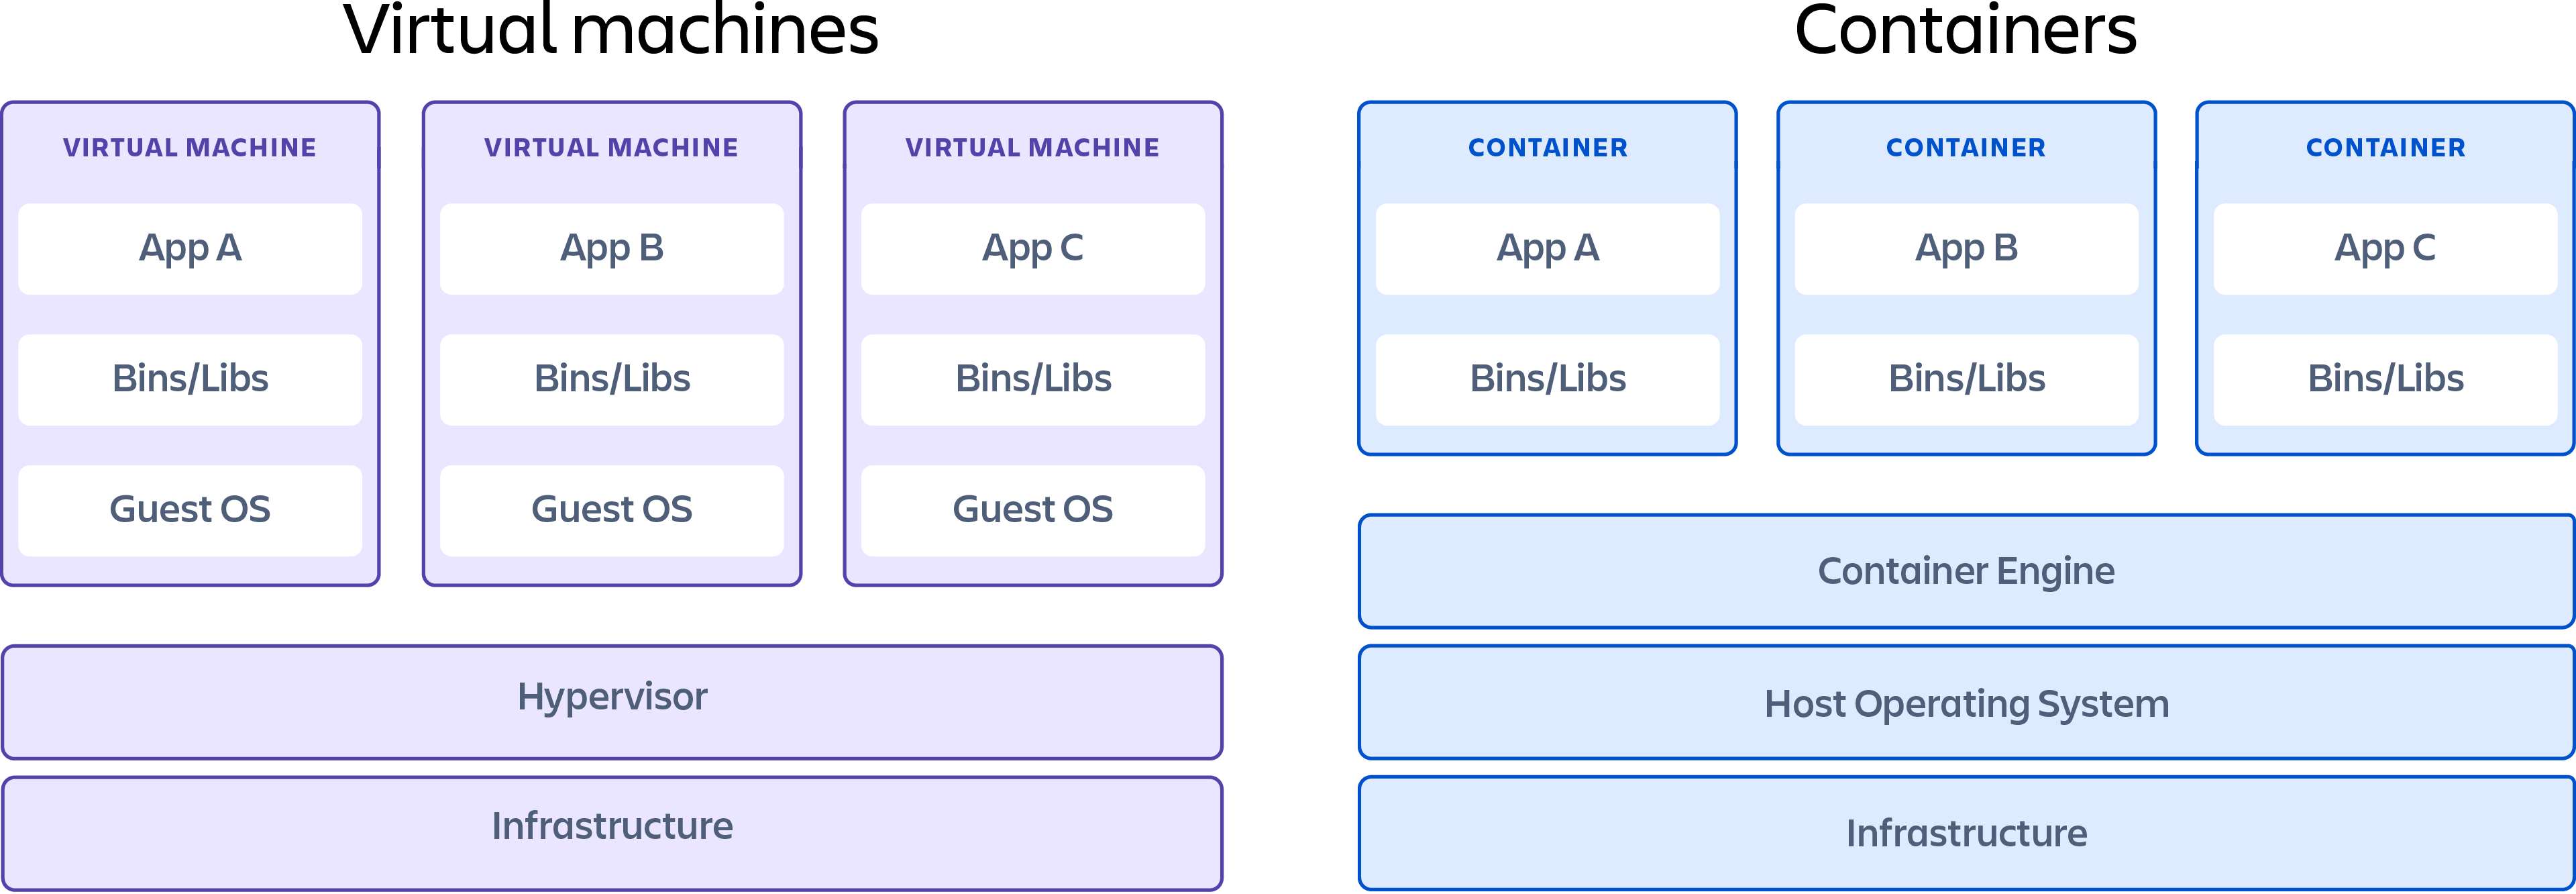
\includegraphics[width=5cm]{image/docker-vs-vm}\footnotemark
            \column{0.5\textwidth}
            Il utilise des outils de la machine, du kernel, \lstinline{chroot} et des librairies de la machine hôte pour fonctionner mais ne fait pas tourner un autre OS contrairement à la virtualisation.
        \end{columns}
        \footnotetext{Containers vs. virtual machines, \url{https://www.atlassian.com/microservices/cloud-computing/containers-vs-vms}}
    \end{frame}

    \begin{frame}
        \transdissolve
        \frametitle{Docker}
        \framesubtitle{Définition}
        Il permet, en théorie, le déploiement de n'importe quelle application sur n'importe quelle architecture (OS, ISA)\footnote{Docker official Images, \url{https://github.com/docker-library/official-images\#architectures-other-than-amd64}}~:
        \bigbreak
        \begin{columns}
            \column{0.4\textwidth}
            \begin{scriptsize}
                \begin{itemize}
                    \item ARMv6 32-bit (arm32v6)
                    \item ARMv7 32-bit (arm32v7)
                    \item ARMv8 64-bit (arm64v8)
                    \item Linux x86-64 (amd64)
                    \item Windows x86-64 (windows-amd64)
                    \item ARMv5 32-bit (arm32v5)
                    \item IBM POWER LE (ppc64le)
                    \item IBM z Systems (s390x)
                    \item MIPS64 LE (mips64le)
                    \item RISC-V 64-bit (riscv64)
                    \item x86/i686 (i386)
                \end{itemize}
            \end{scriptsize}
            \column{0.6\textwidth}
            \centering
            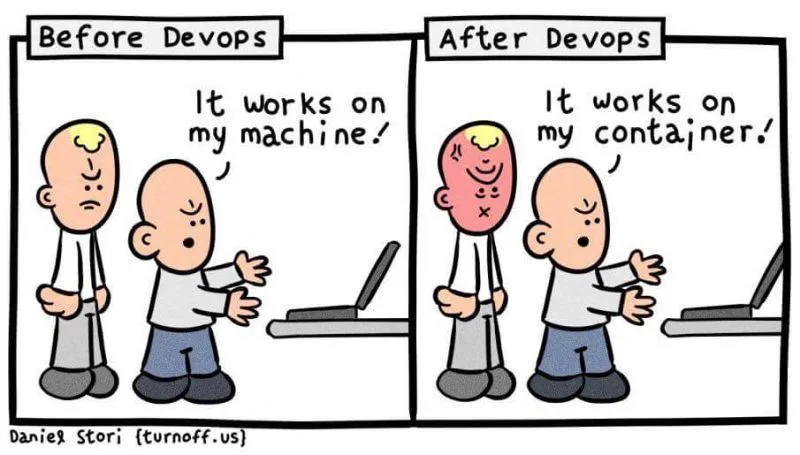
\includegraphics[width=6cm]{image/it-works}
        \end{columns}
    \end{frame}

    \begin{frame}
        \transdissolve
        \frametitle{Docker, créer une image}
        \framesubtitle{Définir l'image dans un Dockerfile}
        L'essentiel de la Dockerfile~:
        \begin{itemize}
            \item Le nom de fichier par convention est \lstinline{Dockerfile} mais peut être différent.
            \item Il vient surcharger une image de base définit dans \lstinline{FROM}.
            \item On peut y définir des variables d'environnement avec \lstinline{ENV}.
            \item La commande \lstinline{RUN} permet d'exécuter des commandes dans l'image.
            Comme par exemple pour ajouter des dépendances dans l'étape de build de l'image.
            \item La commande \lstinline{CMD} définit la commande qui sera exécutée au démarrage du conteneur.
            \item La commande \lstinline{EXPOSE} définit les ports qui seront exposés par le conteneur.
            \item La commande \lstinline{COPY} permet de copier des fichiers dans l'image.
            \item La commande \lstinline{ADD} permet de copier des fichiers dans l'image et de les décompresser.
            \item \textit{Many more\ldots}\footnote{Dockerfile reference, \url{https://docs.docker.com/reference/dockerfile/}}
        \end{itemize}
    \end{frame}

    \begin{frame}[fragile]
        \transdissolve
        \frametitle{Docker, créer une image}
        \framesubtitle{Définir l'image dans un Dockerfile}
        Que fait cette Dockerfile~?
        \begin{lstlisting}[basicstyle=\ttfamily\tiny]
FROM mysql:8-debian

ENV RNCS_PATH=/root/rncs

COPY ./ ${RNCS_PATH}
WORKDIR ${RNCS_PATH}

RUN apt-get update && \
apt-get install -y jq python3 python3-pip moreutils wget unzip libcairo2-dev && \
apt-get clean && \
apt-get autoclean && \
apt-get autoremove -y && \
python3 -m pip install --no-cache-dir -r requirements.txt && \
python3 -m pip install --no-cache-dir -r dev-requirements.txt

EXPOSE 3000/tcp
EXPOSE 5000/tcp
        \end{lstlisting}
        Dans la vraie vie tout est très clair grâce à des commentaires explicites \emoji{smiling-face-with-halo}.
    \end{frame}

    \begin{frame}
        \transdissolve
        \frametitle{Le Docker hub}
        \framesubtitle{\textit{Docker Hub is the world's easiest way to create, manage, and deliver your team's container applications}}
        Encore une fois, inutile de tout recoder.
        On vient en premier lieu trouver une image la plus complète possible pour son application.
        \bigbreak
        Il y a probablement une image pour quasi toutes les stacks existantes.
        \bigbreak
        En terme de cybersécurité, veillez à auditer les développeurs des images pour ne pas subir une \textit{supply chain attack}.

        Une des bonnes pratiques est d'utiliser des images officielles.
        Par exemple pour Tensorflow, le développeur est Google, etc.
        \bigbreak
        Concernant les performances, les images basées sur Alpine Linux sont souvent plus légères car l'OS est développées autour de \lstinline{musl libc} et busybox.
    \end{frame}

    \begin{frame}
        \transdissolve
        \frametitle{Les commandes Docker}
        \framesubtitle{Builder, lancer et stopper une image}
        Ci-dessous, quelques commandes Docker de base~:
        \begin{itemize}
            \item \lstinline{docker build -t <image-name> .} pour construire une image Docker.
            \item \lstinline{docker run <image-name>} pour lancer une image Docker.
            \item \lstinline{docker stop <container-id>} pour arrêter un conteneur.
            \item \lstinline{docker ps} pour lister les conteneurs en cours d'exécution.
            \item \lstinline{docker ps -a} pour lister tous les conteneurs.
            \item \lstinline{docker images} pour lister les images.
            \item \lstinline{docker rmi <image-id>} pour supprimer une image.
            \item \lstinline{docker rm <container-id>} pour supprimer un conteneur.
            \item \lstinline{docker exec -it <container-id> /bin/bash} pour accéder à un conteneur.
        \end{itemize}
    \end{frame}

    \begin{frame}
        \transdissolve
        \frametitle{Docker, créer une image}
        \framesubtitle{Instllation d'un environnement de développement Docker}
        Comme le dit le site Docker, \textit{Build, Share, Run, verify}.
        Tout cela est possible avec Docker Desktop.
        Un GUI qui centralise la plupart des fonctionnalités de Docker.
        \bigbreak
        Sur la machine de production le Docker Engine suffit.
        \bigbreak
        \centering
        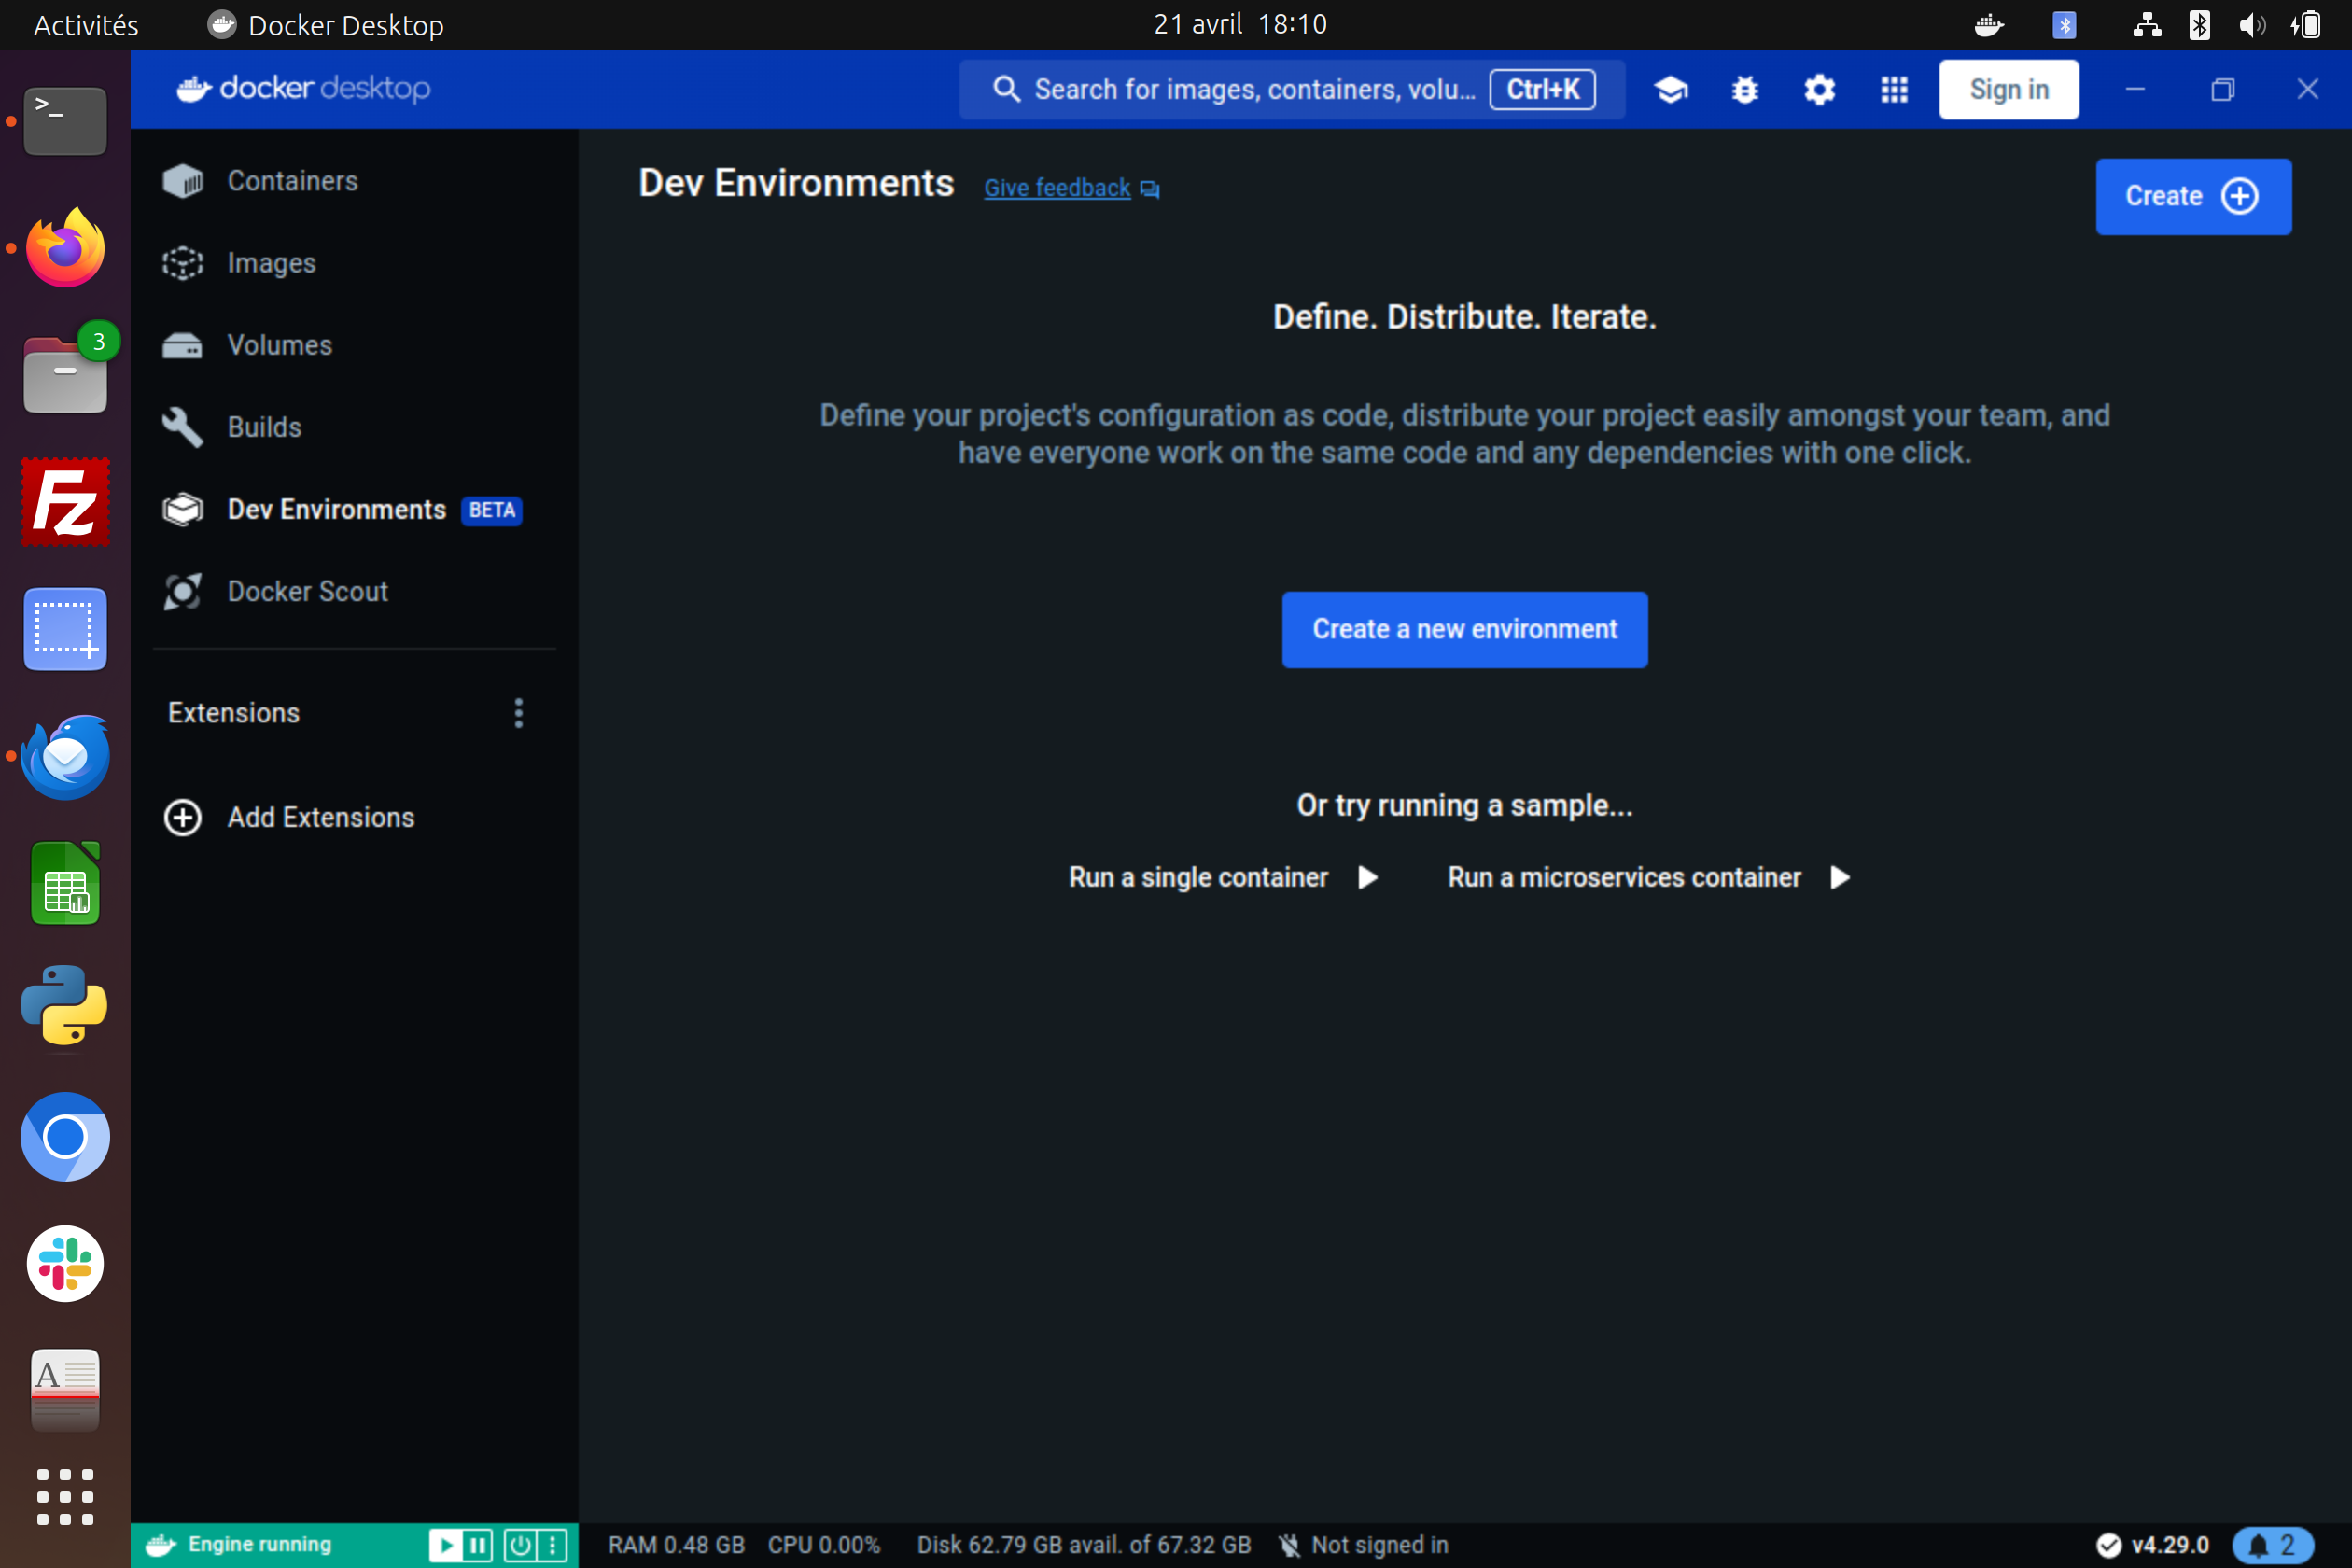
\includegraphics[width=8cm]{image/docker-desktop}
    \end{frame}

    \begin{frame}
        \transdissolve
        \frametitle{Docker, trouver la bonne image}
        \framesubtitle{Exercice}
        Sur le Docker Hub, trouvez les images pour les applications suivantes:
        \begin{itemize}
            \item Une application NodeJS~.
            \item Une application Flask.
            \item OpenJDK 17.
            \item Alpine Linux
        \end{itemize}
    \end{frame}

    \begin{frame}
        \transdissolve
        \frametitle{Docker, créer une image}
        \framesubtitle{Exercice}
        Développer une image Docker pour une application Spring Boot, la même qu'à l'exercice précédent.
        \bigbreak
        Pensez à optimiser l'image pour qu'elle soit la plus légère possible et le plus sécurisé possible\ldots
        \bigbreak
        \centering
        
\includegraphics[width=5cm]{image/young-studying}
    \end{frame}

    \begin{frame}[fragile]
        \transdissolve
        \frametitle{Docker, créer une image}
        \framesubtitle{Une solution possible de l'exercice}
        Avec uniquement une image Eclipse Temurin basée sur une distribution Alpine Linux comme par exemple l'image Docker \textbf{officielle} \lstinline{eclipse-temurin:17-alpine} on génère une image de \textquote{seulement} ~360 Mo\ldots.
        \bigbreak
        \fbox{%
            \begin{minipage}{0.95\textwidth}
                Eclipse Temurin est une JVM maintenue par la Fondation Eclipse, elle offre des performances élevées, la compilation en exécutable et est Java SE TCK (Technology Compatibility Kit).
            \end{minipage}
        }
        \bigbreak
        C'est donc une image de choix en terme de taille, sécurité et performance.
        \begin{lstlisting}
FROM eclipse-temurin:17-alpine # L'image de base
EXPOSE 8081 # Le port du serveur Spring
# Le fichier JAR
COPY helloworld/build/libs/helloworld-0.0.1-SNAPSHOT.jar /app/spring-boot.jar
# Exécution de la JAR
CMD ["java", "-jar", "/app/spring-boot.jar"]
        \end{lstlisting}
    \end{frame}

    \begin{frame}[fragile]
        \transdissolve
        \frametitle{Docker compose}
        \framesubtitle{Le fichier de configuration Docker Compose\footnote{Networking in Compose, \url{https://docs.docker.com/compose/networking/}}}
        Le fichier \lstinline{docker compose.yml} permet de définir comment les conteneurs communiquent entre eux et avec la machine.
        Limiter les ressources CPU et mémoire prise sur la machine.
        \bigbreak
        Pour les applications web par exemple, il faut définir les ports qui seront exposés par les conteneurs~:
        \begin{lstlisting}
services:
  web:
    build: .
    ports:
      - "8000:8000"
  db:
    image: postgres
    ports:
      - "8001:5432"
        \end{lstlisting}
    \end{frame}

    \begin{frame}[fragile]
        \transdissolve
        \frametitle{Docker compose}
        \framesubtitle{Le fichier de configuration Docker Compose\footnote{Compose Build Specification, \url{https://docs.docker.com/compose/compose-file/build/}]}}
        On y définit aussi le(s) Dockerfile(s)~:
        \begin{lstlisting}
version: "3"

services:
  client:
    build:
      context: ../
      dockerfile: docker/Dockerfile.production
        \end{lstlisting}
    \end{frame}

    \begin{frame}[fragile]
        \transdissolve
        \frametitle{Docker compose}
        \framesubtitle{Le fichier de configuration Docker Compose\footnote{docker compose, \url{https://docs.docker.com/reference/cli/docker/compose/}}}
        Les commandes pour builder, lancer et stopper les conteneurs définis dans le fichier \lstinline{docker-compose.yml}~:
        \begin{itemize}
            \item \lstinline{docker compose build} pour construire les images.
            \item \lstinline{docker compose up} pour lancer les conteneurs.
            \item \lstinline{docker compose down} pour arrêter les conteneurs.
            \item \lstinline{docker compose ps} pour lister les conteneurs en cours d'exécution.
            \item \lstinline{docker compose ps -a} pour lister tous les conteneurs.
            \item \lstinline{docker compose images} pour lister les images.
            \item \lstinline{docker compose exec <container-name> /bin/bash} pour accéder à un conteneur.
        \end{itemize}
        Elles sont très similaires aux commandes Docker.
    \end{frame}

    \begin{frame}[fragile]
        \transdissolve
        \frametitle{Docker compose}
        \framesubtitle{Exercice, développer une configuration Docker Compose}
        Un Docker compose pour un site Wordpress, ce dernier a besoin d'une base de données MySQL~.
        \pause
        \begin{lstlisting}[basicstyle=\ttfamily\tiny]
services:
  db:
    image: 'mysql:8'
    env_file:
      - .env
    volumes:
      - 'db_data:/var/lib/mysql'
    restart: always
    environment:
      MYSQL_ROOT_PASSWORD: k36FbP3NH3J8
      MYSQL_DATABASE: ${WORDPRESS_DB_USER}
      MYSQL_USER: ${WORDPRESS_DB_USER}
      MYSQL_PASSWORD: ${WORDPRESS_DB_PASSWORD}
  wordpress:
    depends_on:
      - db
    image: 'wordpress:latest'
    ports:
      - '8000:80'
    restart: always
    environment:
      WORDPRESS_DB_HOST: 'db:3306'
      WORDPRESS_DB_USER: ${WORDPRESS_DB_USER}
      WORDPRESS_DB_PASSWORD: ${WORDPRESS_DB_PASSWORD}
volumes:
  db_data: null
        \end{lstlisting}
    \end{frame}

    \begin{frame}[fragile]
        \transdissolve
        \frametitle{Docker compose}
        \framesubtitle{Exercice, développer une configuration Docker Compose}
        Des variables d'environnement comme les mots de passe, etc, sont définies dans un fichier \lstinline{.env}.
        \bigbreak
        Pas de build de Dockerfile donc une seule commande suffit pour lancer Wordpress~:
        \begin{lstlisting}[language=bash]
$ docker compose up
        \end{lstlisting}
    \end{frame}


    \section{Kubernetes}\label{sec:kubernetes}

    \begin{frame}
        \transdissolve
        \frametitle{Kubernetes}
        \framesubtitle{Définition et histoire\footnote{Qu'est ce que Kubernetes, \url{https://kubernetes.io/fr/docs/concepts/overview/what-is-kubernetes/}}}
        \begin{columns}
            \column{0.5\textwidth}
            Kubernetes est un orchestrateur de conteneurs open-source.
            Il permet de déployer, de gérer et de \textbf{scaler} des applications conteneurisées.
            \bigbreak
            Créé et libéré en open source par Google en 2014, il est maintenant maintenu par la Cloud Native Computing Foundation (CNCF) de la Linux Foundation.
            \bigbreak
            Aussi appelé par son abréviation \textquote{K8s} comme k de K, 8 lettres puis un s.
            \column{0.5\textwidth}
            \centering
            
\includegraphics[width=6cm]{image/kubernetes-logo}
        \end{columns}
    \end{frame}

    \begin{frame}
        \transdissolve
        \frametitle{Kubernetes}
        \framesubtitle{Les termes clés\footnote{\label{k8soracle}Qu’est-ce que Kubernetes ?, \url{https://www.oracle.com/fr/cloud/cloud-native/container-engine-kubernetes/what-is-kubernetes/}}}
        \begin{itemize}
            \item \textbf{Cluster}~: Ensemble de machines, appelées individuellement « nœuds », utilisées pour exécuter des applications conteneurisées gérées par Kubernetes.
            \item \textbf{Node}~: Il s'agit d'une machine virtuelle ou physique.
            Un cluster se compose d'un nœud maître et de plusieurs nœuds de travail.
            \item \textbf{Pod}~: Conteneur unique ou ensemble de conteneurs s’exécutant sur un cluster Kubernetes.
            \item \textbf{Volume}~: Un répertoire qui contient des données accessibles par les conteneurs.
            \item \textbf{Deployment}~: Objet qui gère les applications répliquées représentées par des pods.
            Les pods sont déployés sur les nœuds d’un cluster.
        \end{itemize}
    \end{frame}

    \begin{frame}
        \transdissolve
        \frametitle{Kubernetes}
        \framesubtitle{Kubernetes Components\footnote{\label{k8scompnents}Kubernetes – Introduction à l’architecture et aux composants, \url{https://kubernetes.io/docs/concepts/overview/components/}}}
        \begin{itemize}
            \item \textbf{kube-apiserver}~: Composant central qui fournit l'API Kubernetes.
            \item \textbf{etcd}~: Stockage de données clé-valeur.
            \item \textbf{kube-scheduler}~: Ordonnanceur qui distribue les pods sur les nœuds.
            \item \textbf{kube-controller-manager}~: Composant qui exécute les contrôleurs.
            \item \textbf{kubelet}~: Agent qui s'exécute sur chaque nœud du cluster.
            Il s'assure que les conteneurs sont en cours d'exécution dans un pod.
            \item \textbf{Kube-proxy}~: Proxy réseau qui s'exécute sur chaque nœud du cluster.
            \item \textbf{Container runtime}~: Gère les exécutions de manière \textquote{efficace} et leur cycle de vie des conteneurs dans l'environnement K8s.
        \end{itemize}
    \end{frame}

    \begin{frame}
        \transdissolve
        \frametitle{Kubernetes}
        \framesubtitle{Architectures\cref{k8scompnents}}
        \centering
        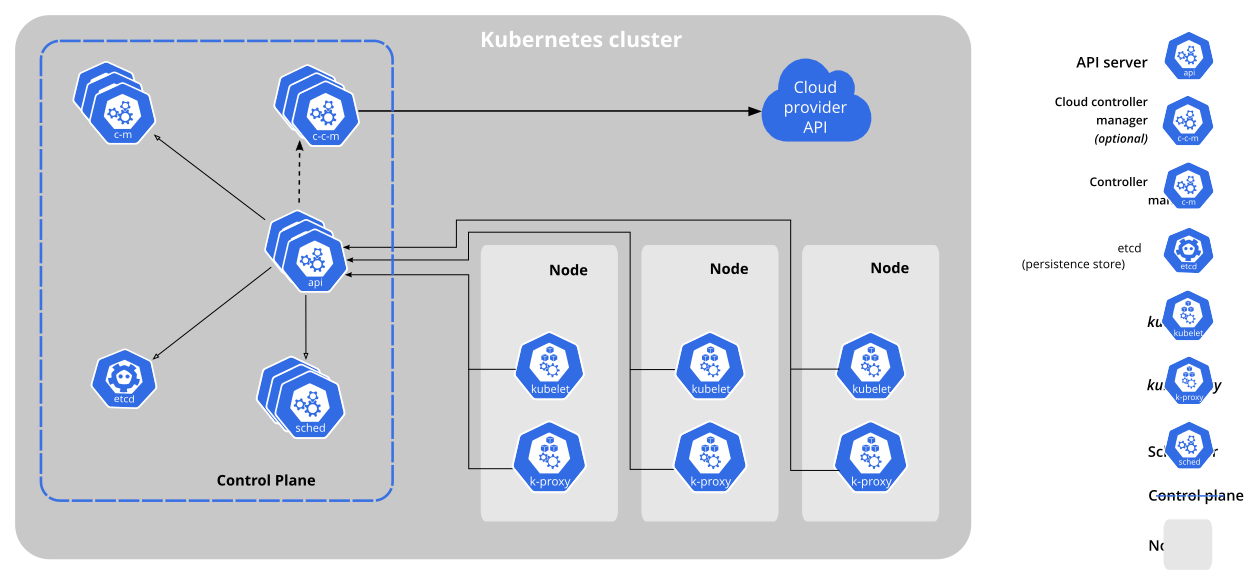
\includegraphics[width=10cm]{image/components-of-kubernetes}
    \end{frame}

    \begin{frame}
        \transdissolve
        \frametitle{Kubernetes}
        \framesubtitle{Addons et third party\footnote{Installing Addons, \url{https://kubernetes.io/docs/concepts/cluster-administration/addons/}}}
        Développé par la communauté Kubernetes, ils apportent des fonctionnalités supplémentaires à Kubernetes.
        Comme par exemple l'add-on registry qui permet de stocker les images des conteneurs\footnote{How to use the built-in registry, \url{https://microk8s.io/docs/registry-built-in}}.
        \bigbreak
        Ceux proposés par la documentation officielle \url{https://kubernetes.io/docs/concepts/cluster-administration/addons/}.

        D'autres sont disponibles sur le \href{https://hub.kubeapps.com/}{Kubeapps} une application Kubernetes.
        \bigbreak
        Mais bien d'autres ont été mis en open source, pas de ledger unique trouvé à l'heure actuelle.
    \end{frame}

    \begin{frame}
        \transdissolve
        \frametitle{Kubernetes}
        \framesubtitle{Les types de conteneurs supportés\footnote{Container Runtimes, \url{https://kubernetes.io/docs/setup/production-environment/container-runtimes/}}}
        Kubernetes supporte plusieurs runtimes de conteneurs~:
        \begin{itemize}
            \item Docker
            \item Containerd
            \item CRI-O
            \item Mirantis Container Runtime
        \end{itemize}
    \end{frame}

    \begin{frame}
        \transdissolve
        \frametitle{Kubernetes}
        \framesubtitle{Les interfaces}
        \begin{columns}
            \column{0.5\textwidth}
            Le dashboard Kubernetes est une interface web qui permet de gérer les ressources du cluster\footnotemark.
            \column{0.5\textwidth}
            \centering
            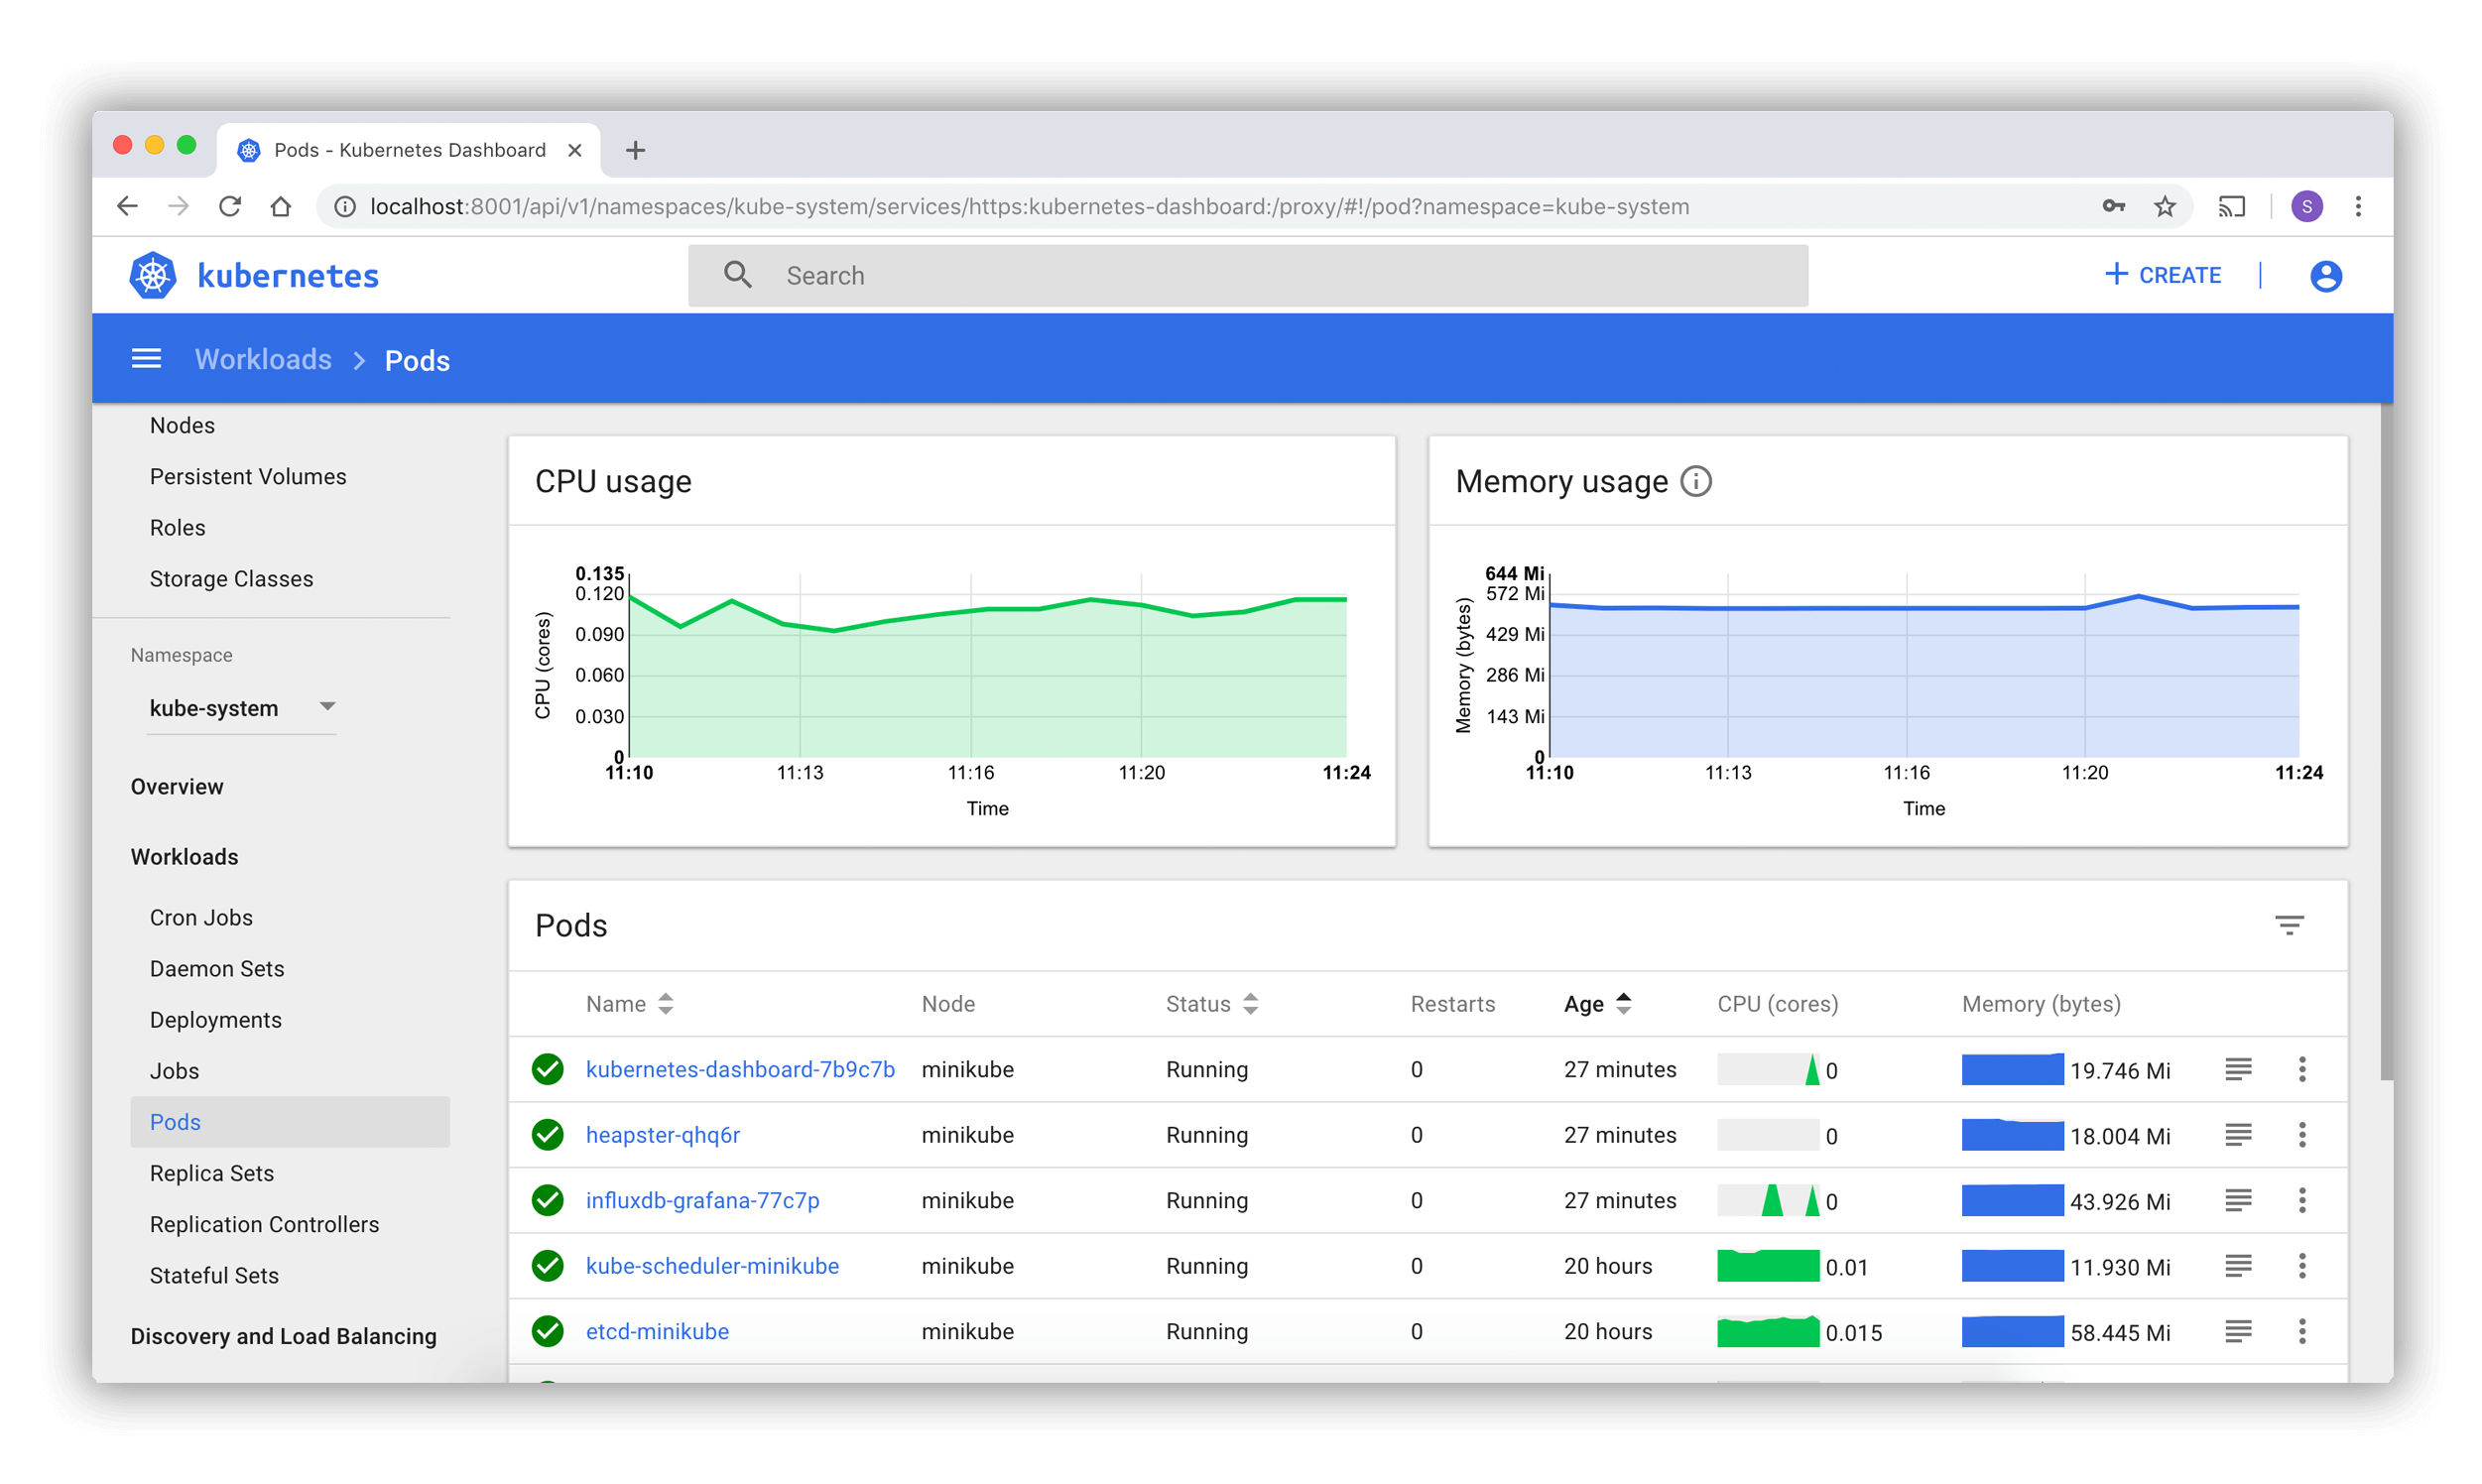
\includegraphics[width=5cm]{image/kubernetes-dashboard}
        \end{columns}
        \footnotetext{Container Runtimes, \url{https://kubernetes.io/fr/docs/tasks/access-application-cluster/web-ui-dashboard/}}
        \flushleft
        \bigbreak
        Il existe également une CLI, \lstinline{kubectl} qui permet de gérer le cluster, elle utilise la Kubernetes API\footnote{\url{https://kubernetes.io/docs/reference/kubectl/}}.
        \bigbreak
        La Kubernetes API qui rend le cluster accessible depuis la plupart des langages de programmation.
    \end{frame}

    \begin{frame}
        \transdissolve
        \frametitle{Kubernetes}
        \framesubtitle{Les différentes versions\footnote{How to deploy Kubernetes, \url{https://ubuntu.com/kubernetes/install}}}
        Il existe plusieurs distributions de Kubernetes~:
        \begin{itemize}
            \item \textbf{MicroK8s} pour des clusters de petites et moyenne taille.
            \item \textbf{Charmed Kubernetes} pour des cluster moyen et gros.
            \item \textbf{Kubeadm} un DIY Kubernetes configurable.
            \item Many more\ldots
        \end{itemize}
    \end{frame}

    \begin{frame}
        \transdissolve
        \frametitle{Infrastructure Kubernetes de St-Michel}
        \framesubtitle{Instance Micro-K8s dédiée aux exercices}
        \bigbreak
        \centering
        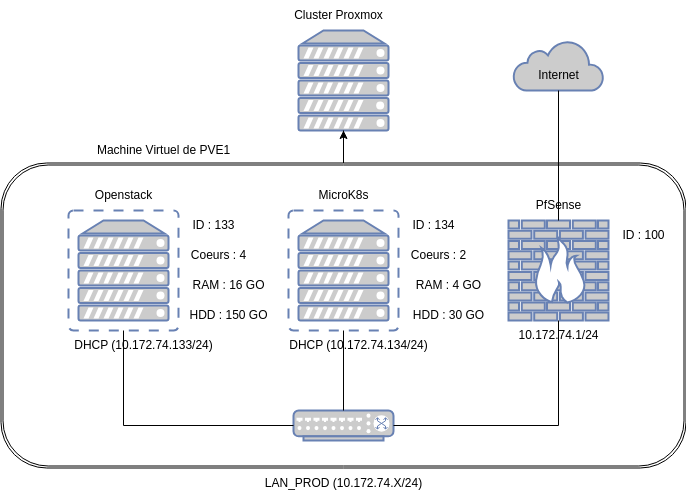
\includegraphics[width=10cm]{image/infra.drawio}
    \end{frame}

    \begin{frame}
        \transdissolve
        \frametitle{Exercice de déploiement dans Kubernetes}
        \framesubtitle{Exercice évalué sur le déploiement d'une application Spring Boot dans Kubernetes}
        Pousser l'image sur le registry de MicroK8s et exécuter l'application Spring Boot \textquote{Dockerisée} de l'avant dernier exercice dans le MicroK8s de la VM du cluster Proxmox.
        \bigbreak
        L'application doit être accessible sur le réseau de St-Michel.
        \bigbreak
        \centering
        
\includegraphics[width=5cm]{image/maniac-programmer-sorting-her-code}
    \end{frame}

    \begin{frame}[fragile]
        \transdissolve
        \frametitle{Exercice de déploiement dans Kubernetes}
        \framesubtitle{Solution de l'exercice}
        L'image est buildée et tagger sur la machine du développeur~:
        \begin{lstlisting}[language=bash]
$ docker build -t 10.172.74.134:32000/my-fancy-app:1.0.0 .
        \end{lstlisting}
        Poussée sur le registry de MicroK8s~:
        \begin{lstlisting}[language=bash]
$ docker push 10.172.74.134:32000/my-fancy-app:1.0.0
The push refers to repository [10.172.74.134:32000/my-fancy-app]
0c4cac1d4e27: Pushed
5a8f0ac5756e: Pushed
...
        \end{lstlisting}
        Configuration du déploiement dans la web UI~:
        \begin{columns}
            \column{0.5\textwidth}
            \centering
            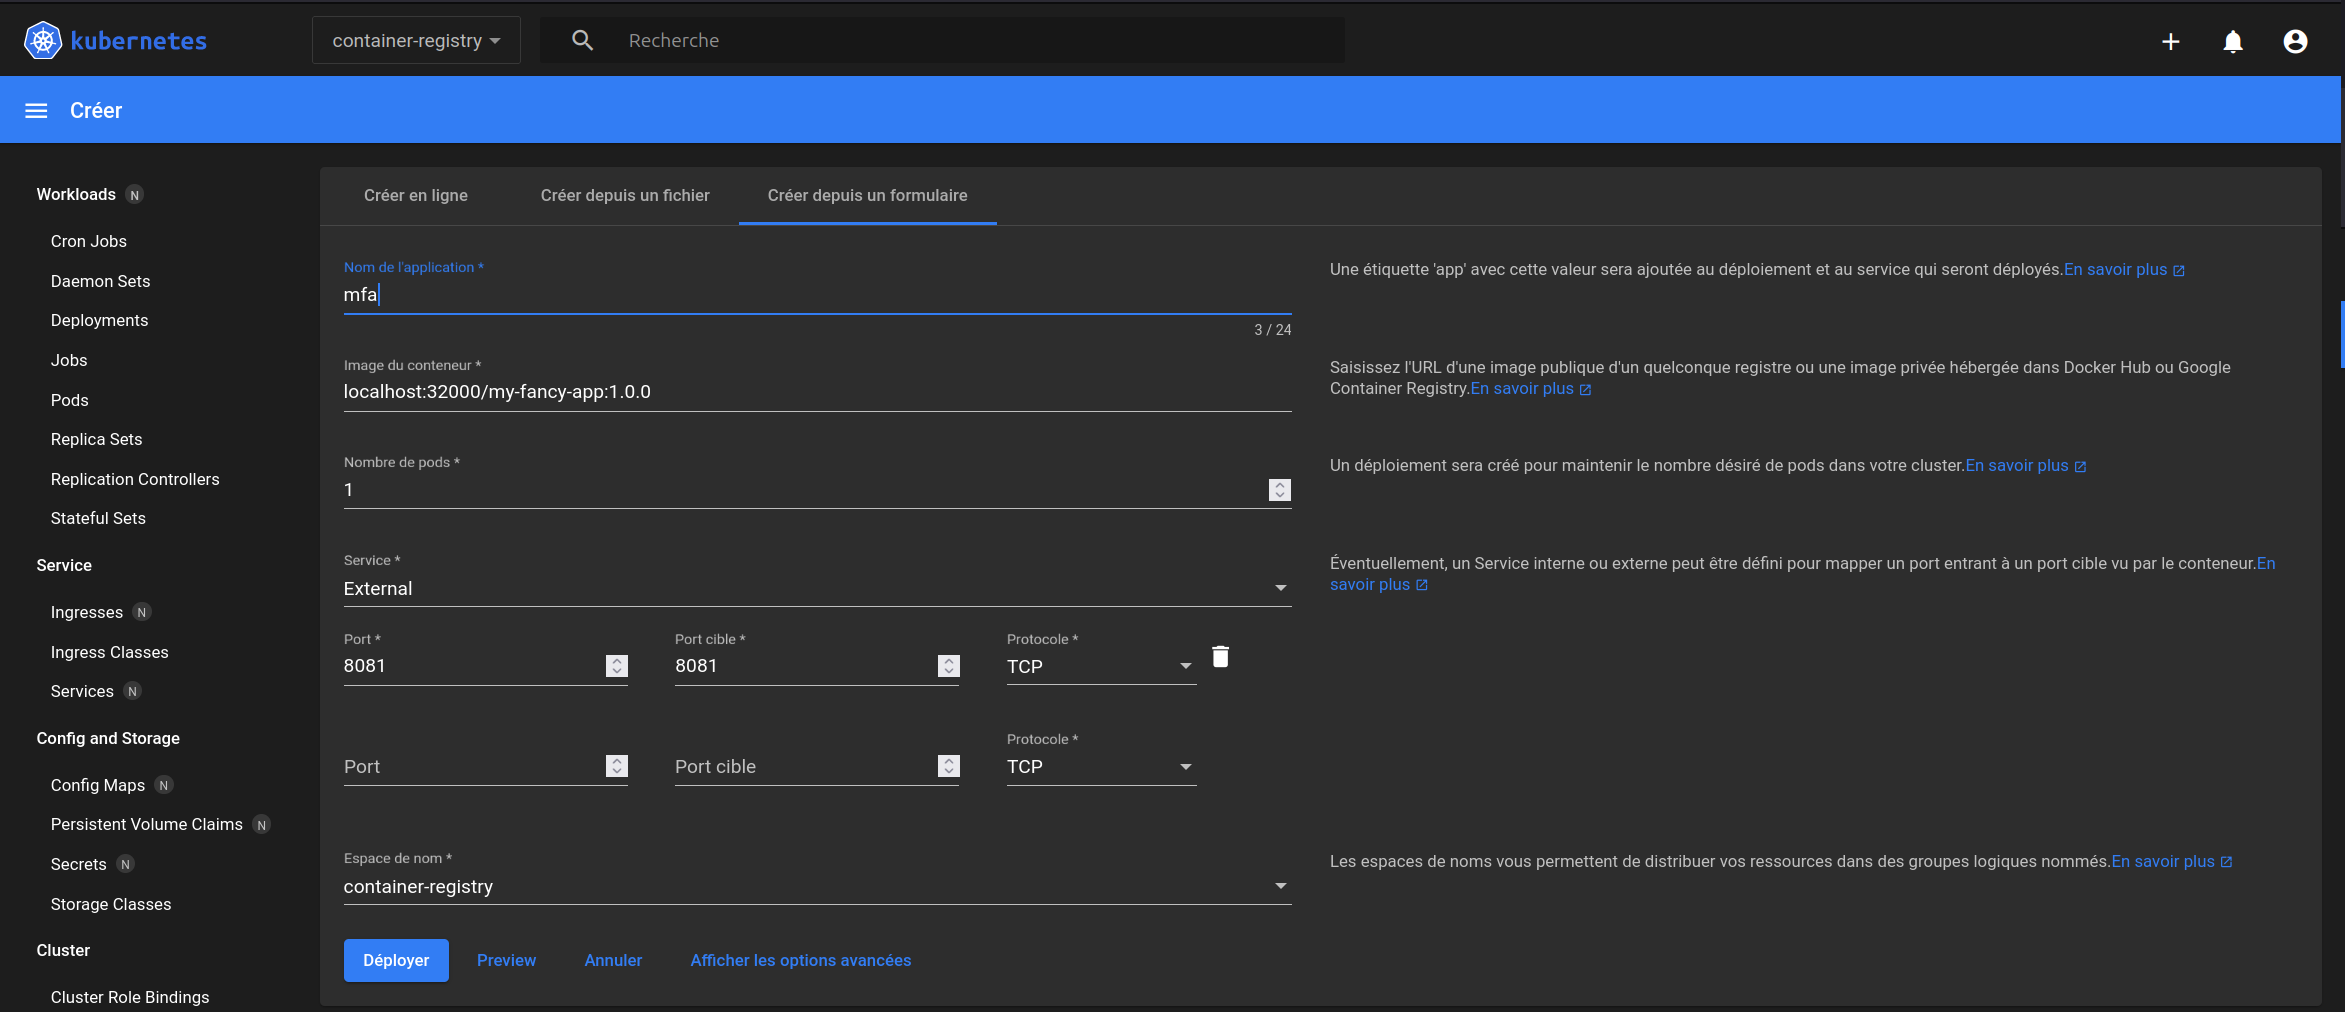
\includegraphics[width=5.5cm]{image/k8s-deployment-configuration}
            \column{0.5\textwidth}
            \centering
            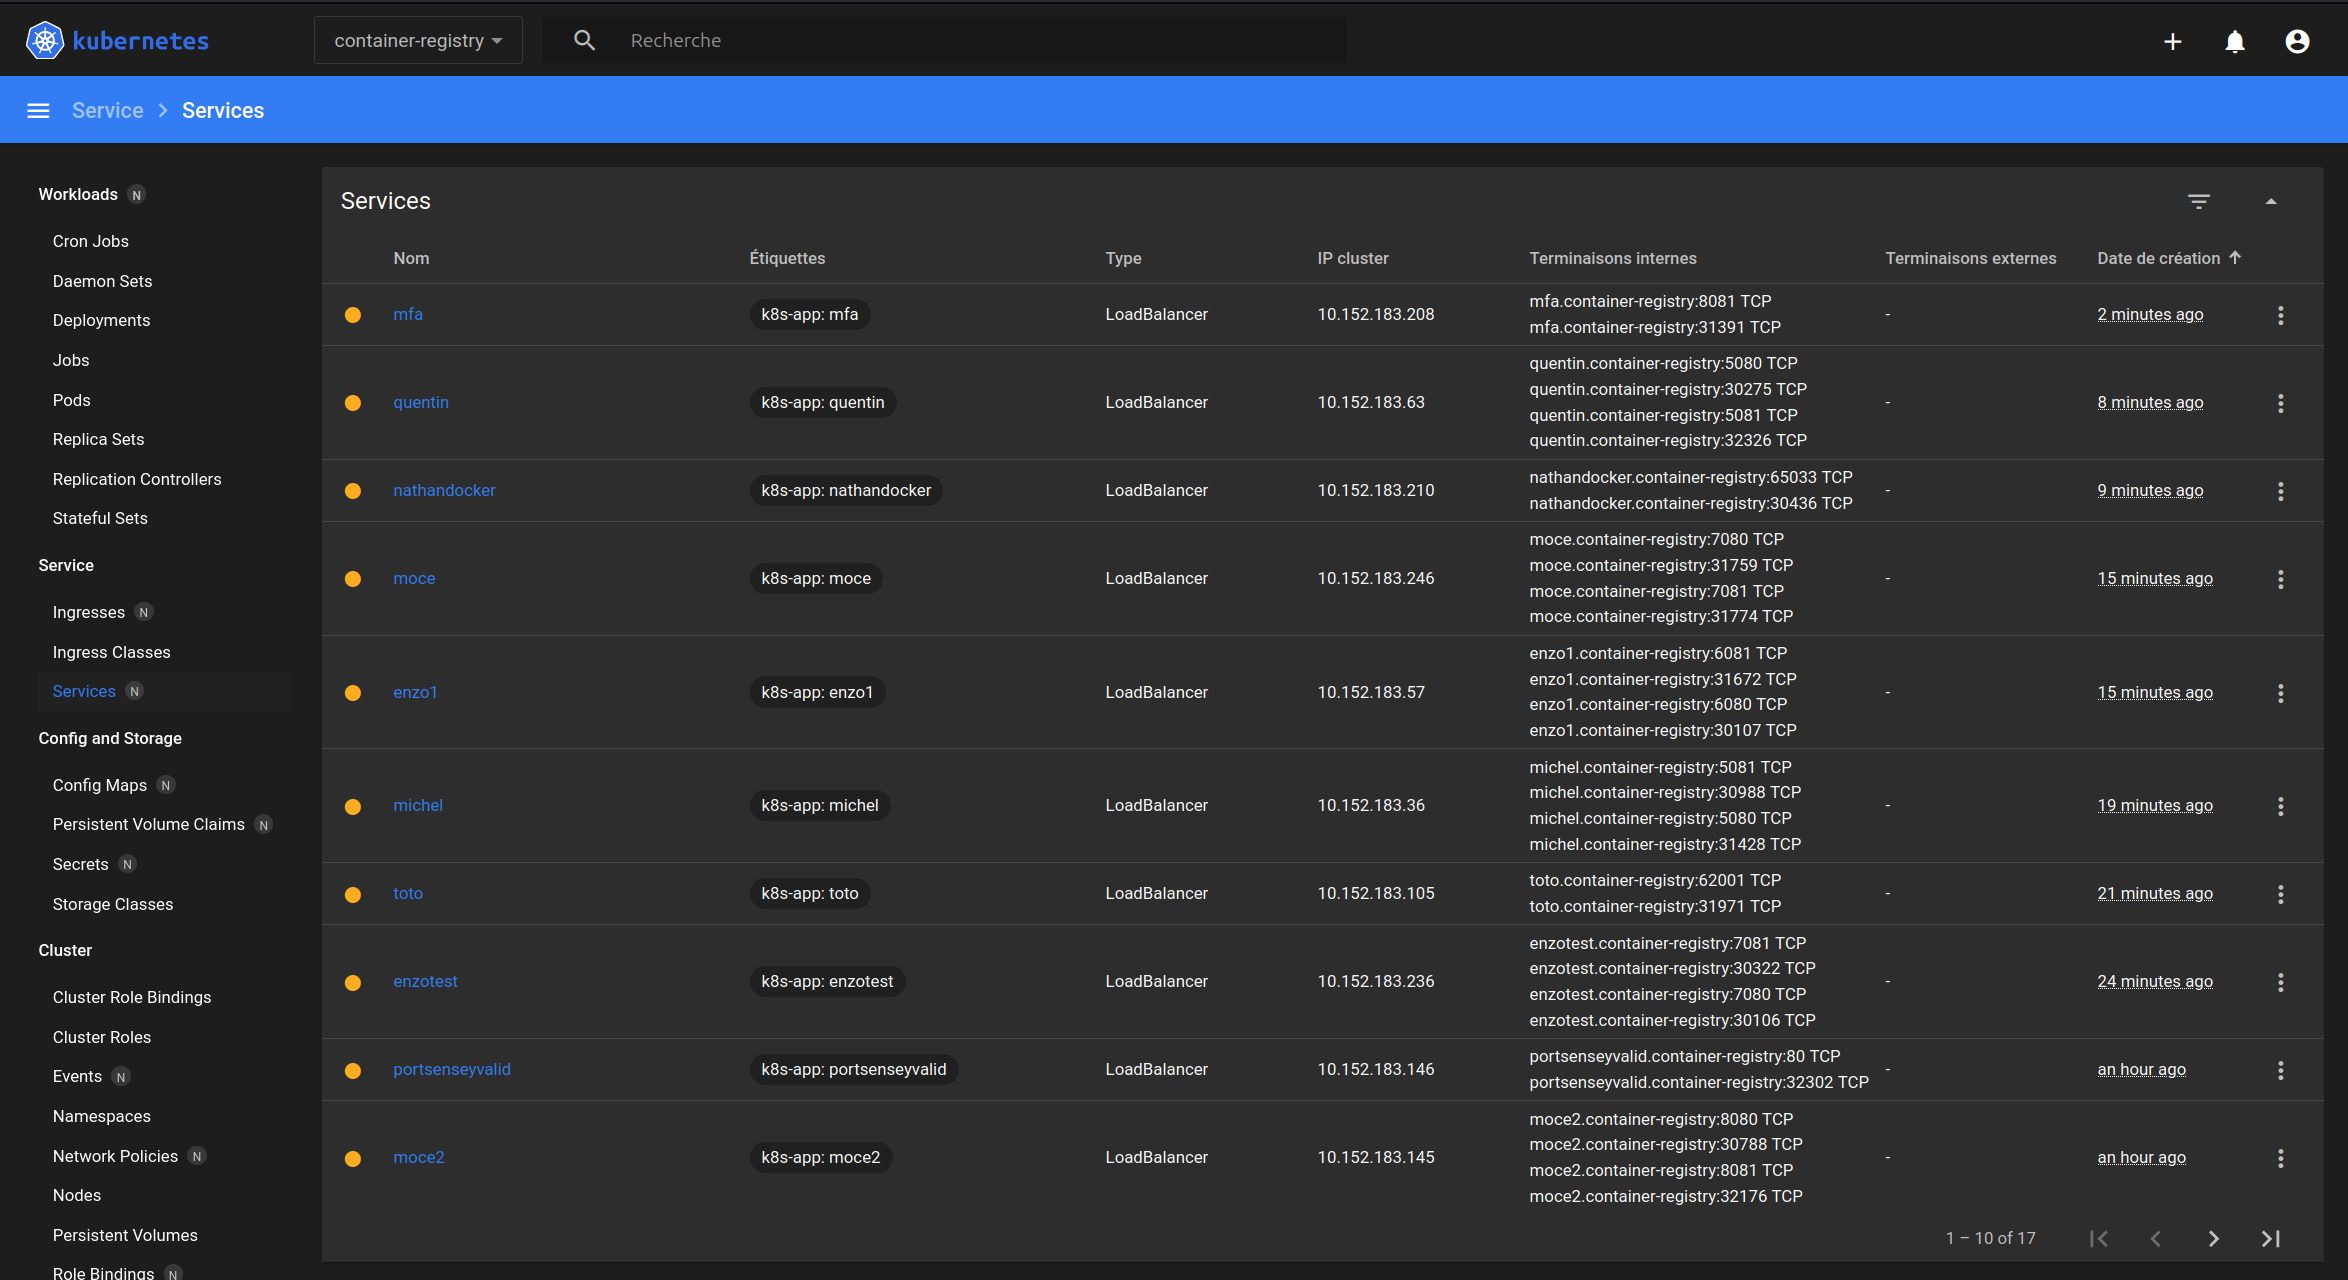
\includegraphics[width=5.5cm]{image/k8s-services}
        \end{columns}
    \end{frame}


    \section{OpenStack}\label{sec:openstack}

    \begin{frame}
        \transdissolve
        \frametitle{OpenStack}
        \framesubtitle{Définition\footnote{\label{OpenStackhome}OpenStack, \url{https://www.OpenStack.org/}}}
        C'est un logiciel de gestion de cloud, un \textquote{Cloud software}.
        On peut aussi dire que c'est un OS de cloud.
        \bigbreak
        \textquote{OpenStack is a set of software components that provide common services for cloud infrastructure.}
        \bigbreak
        \textquote{Cloud Infrastructure for Virtual Machines, Bare Metal, and Containers}.
        \bigbreak
        \textquote{OpenStack controls large pools of compute, storage, and networking resources, all managed through APIs or a dashboard.}
        \bigbreak
        Il est en open source sous licence Apache 2.0 \textquote{OpenStack is developed by the community. For the community...}.
    \end{frame}

    \begin{frame}
        \transdissolve
        \frametitle{OpenStack}
        \framesubtitle{Définition\cref{OpenStackhome}}
        \bigbreak
        \centering
        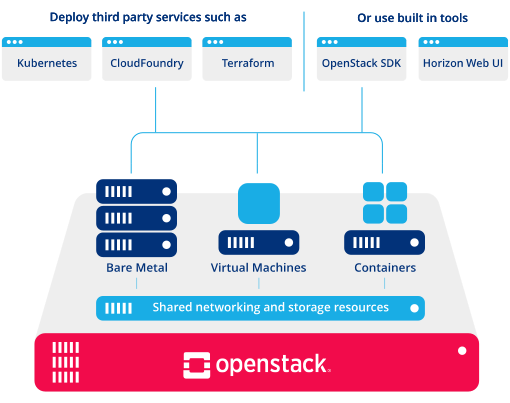
\includegraphics[width=8cm]{image/openstack-overview}
    \end{frame}

    \begin{frame}
        \transdissolve
        \frametitle{OpenStack}
        \framesubtitle{Histoire\footnote{Introduction: A Bit of OpenStack History, \url{https://docs.OpenStack.org/project-team-guide/introduction.html}}}

        \begin{columns}
            \column{0.7\textwidth}
            Né de la convergence des travaux de Rackspace Technology et de la NASA en 2010.
            \bigbreak
            La mission initiale est \textquote{to produce a ubiquitous Open Source Cloud Computing platform that is easy to use, simple to implement, interoperable between deployments, works well at all scales, and meets the needs of users and operators of both public and private clouds}.
            \column{0.3\textwidth}
            \centering
            
\includegraphics[width=3cm]{image/openstack-supports} \\ \tiny{Une partie des supports en 2024}\\
        \end{columns}
    \end{frame}

    \begin{frame}
        \transdissolve
        \frametitle{OpenStack}
        \framesubtitle{Les composants principaux}
        C'est un ensemble services, de composants qui s'assemblent de manière \textquote{plug and play} en fonction des besoins.
        Encore une fois, c'est modulaire\ldots
        \bigbreak
        \centering
        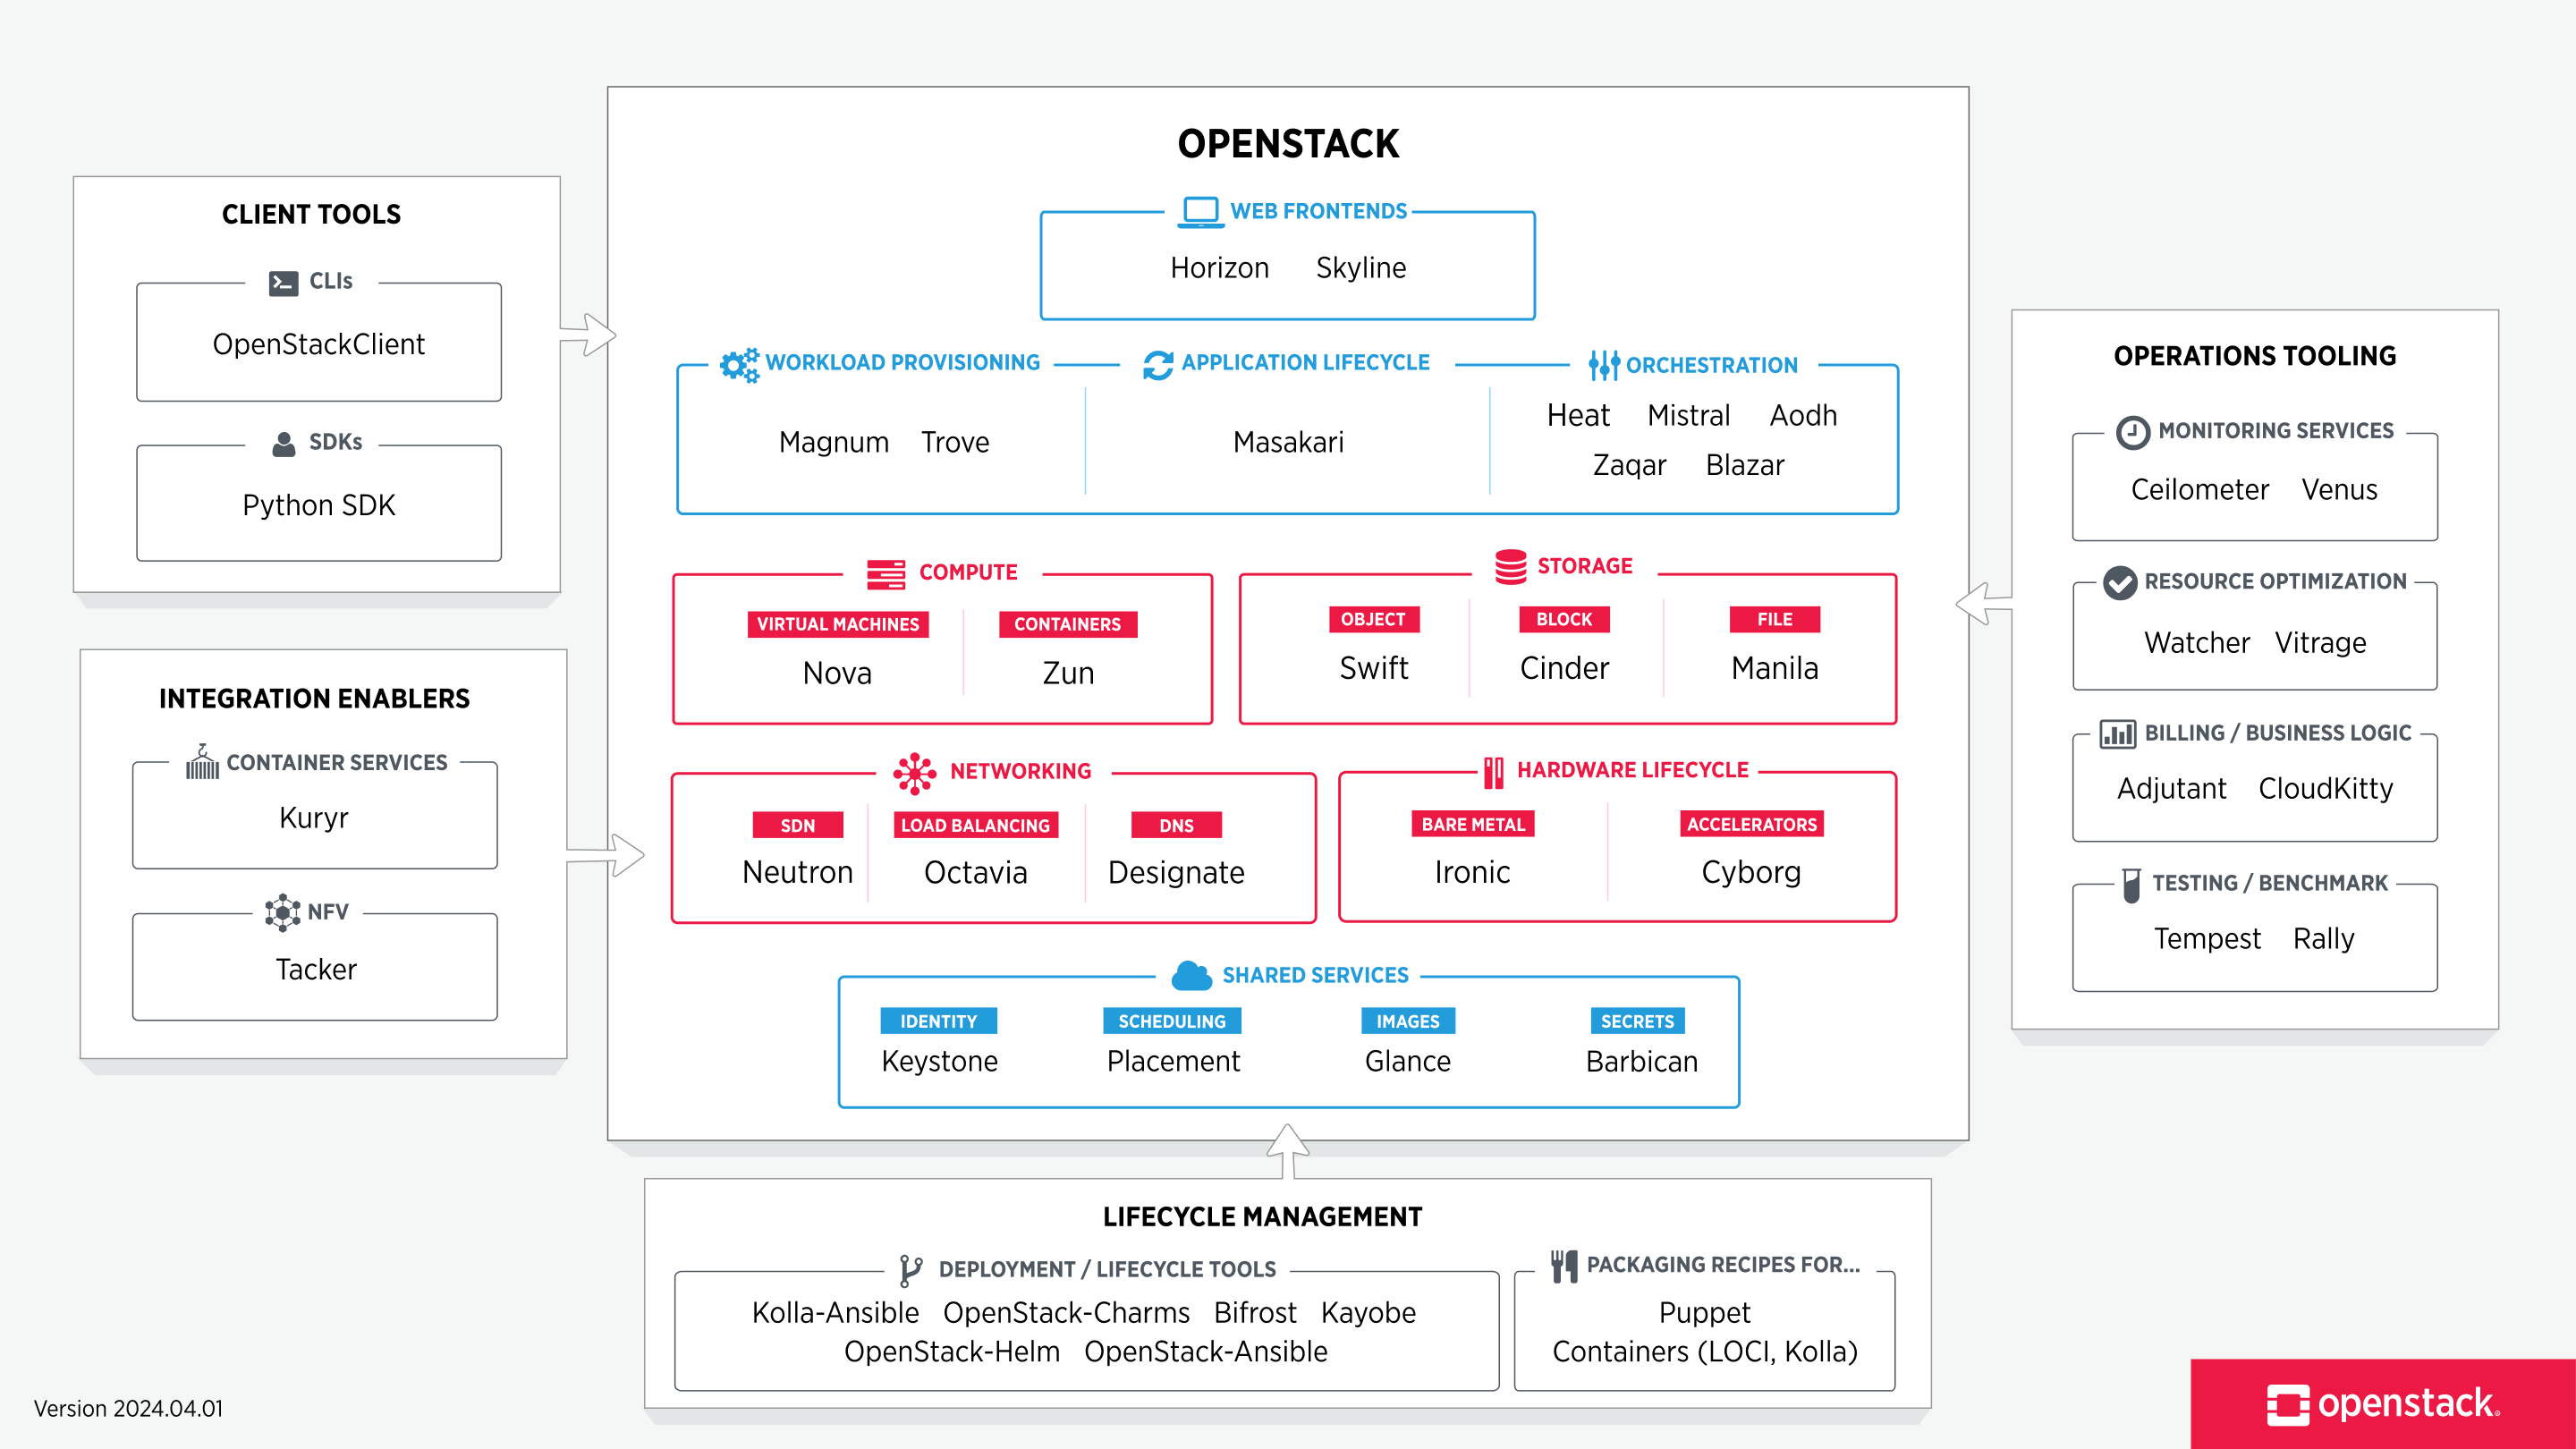
\includegraphics[width=9cm]{image/openstack-components}
        \bigbreak
        \flushleft
        La liste complète des composants est sur le \href{https://www.OpenStack.org/software/project-navigator/OpenStack-components\#OpenStack-services}{site officiel}.
    \end{frame}

    \begin{frame}
        \transdissolve
        \frametitle{OpenStack}
        \framesubtitle{Les interfaces\footnote{\label{OpenStackservices}OpenStack Services, \url{https://www.OpenStack.org/software/project-navigator/OpenStack-components\#OpenStack-services}}\footnote{Client tools, \url{https://www.OpenStack.org/software/project-navigator/sdks}}}
        Les UI web~:
        \begin{itemize}
            \item \textbf{Horizon}~: Le tableau de bord web d'OpenStack.
            \item \textbf{Skyline}~: \textquote{Next generation dashboard}.
        \end{itemize}
        \bigbreak
        Une CLI à installer avec \lstinline{pip install python-OpenStackclient}.
        \bigbreak
        Un SDK Python pour les APIs OpenStack.
    \end{frame}

    \begin{frame}
        \transdissolve
        \frametitle{OpenStack}
        \framesubtitle{Résumé des fonctionnalités\footnote{\label{redhatopentack}OpenStack, qu'est-ce que c'est ?, \url{https://www.redhat.com/fr/topics/OpenStack}}}
        \begin{itemize}
            \item Permet de gérer des clouds privés ou publics.
            \item Virtualisation des ressources.
            \item Stockage objet, bloc et fichier avec \textbf{Swift} et \textbf{Cinder}.
            \item L'authentification et les autorisations avec \textbf{Keystone}.
            \item Le réseau avec \textbf{Neutron}.
            \item Les ressources de calcul avec \textbf{Nova}.
            \item Gestion des conteneurs (Docker entre autre) avec \textbf{Zun}.
        \end{itemize}
    \end{frame}

    \begin{frame}[fragile]
        \transdissolve
        \frametitle{OpenStack}
        \framesubtitle{Commandes de base\footnote{\label{opentackcommand}OpenStack, qu'est-ce que c'est ?, \url{https://www.redhat.com/fr/topics/OpenStack}}}
        Pour ajouter une image à OpenStack~:
        \begin{lstlisting}
$ OpenStack image create <IMAGE> --disk-format raw \
  --container-format bare --public \
  --file ~/images/cirros-0.3.5-x86_64-disk.img
        \end{lstlisting}
        Pour créer un type d'instance, appelé \textquote{flavor}~:
        Pour lancer une instance~:
        \begin{lstlisting}
OpenStack flavor create --ram 512 --disk 1 --vcpus 1 <FLAVOR INSTANCE_NAME>
        \end{lstlisting}
        Pour lancer une instance~:
        \begin{lstlisting}
$ OpenStack server create --image <IMAGE> --flavor <FLAVOR INSTANCE_NAME>
        \end{lstlisting}
        \bigbreak
        Toutes les commandes dans la \href{https://docs.OpenStack.org/ocata/user-guide/cli-cheat-sheet.html}{documentation officielle}.
    \end{frame}
    \begin{frame}
        \transdissolve
        \frametitle{Infrastructure OpenStack de St-Michel}
        \framesubtitle{Instance OpenStack dans une VM dédiée aux exercices}
        \bigbreak
        \centering
        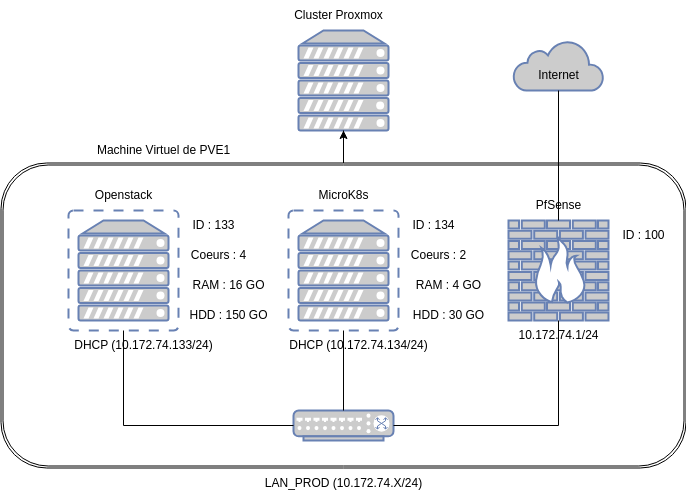
\includegraphics[width=10cm]{image/infra.drawio}
    \end{frame}
    \begin{frame}
        \transdissolve
        \frametitle{OpenStack}
        \framesubtitle{Exercice}
        \begin{itemize}
            \item Créer l'image de l'application Spring Boot dans OpenStack.
            \item Créer un flavor de 1 vCPU et 1 Go de RAM~.
            \item Lancer une instance de l'application Spring Boot.
            \item Faire un snapshot de l'instance.
            \item Stopper l'instance.
            \item Relancer l'instance.
        \end{itemize}
        Réalisez ces tâches avec la CLI OpenStack et listez les commandes pour l'évaluation.
    \end{frame}

    \begin{frame}
        \transdissolve
        \frametitle{OpenStack}
        \framesubtitle{Exercice}
        \begin{itemize}
            \item Créer un registre de conteneur dans OpenStack.
            \item Pousser le conteneur de l'application Spring Boot dans le registre OpenStack.
            \item Lancer un conteneur de l'application Spring Boot avec 1 vCPU et 1 Go de RAM maximum.
            \item Stopper le conteneur.
        \end{itemize}
        Réalisez ces tâches avec la CLI OpenStack et listez les commandes pour l'évaluation.
    \end{frame}

\end{document}
